\documentclass[
	letterpaper, % Paper size, specify a4paper (A4) or letterpaper (US letter)
	10pt, % Default font size, specify 10pt, 11pt or 12pt
]{CSUniSchoolLabReport}

\DeclareSIUnit \siemen {S}

%----------------------------------------------------------------------------------------
%	REPORT INFORMATION
%----------------------------------------------------------------------------------------

\title{Lab Three\\ Fundamentals of Electronics \\ EECE2412/3} % Report title

\author{Michael \textsc{Brodskiy}\\ \small \href{mailto:Brodskiy.M@Northeastern.edu}{Brodskiy.M@Northeastern.edu}}

\date{November 12, 2024} % Date of the report

%----------------------------------------------------------------------------------------


\begin{document}

\maketitle % Insert the title, author and date using the information specified above

\begin{center}
	\begin{tabular}{l r}
        Date Performed: & Oct. 29/Nov. 05, 2024 \\ % Date the experiment was performed
        Partner: & Rahul \textsc{Singh} \\ % Partner names
		Instructor: & Professor \textsc{Onabajo} \\ % Instructor/supervisor
        TAs: & Ming \textsc{Xiang} \& Amr \textsc{Kassab} \\ % Teachers Assistants 
	\end{tabular}
\end{center}

\newpage

\begin{abstract}

  The purpose of this laboratory experiment is to familiarize ourselves with bipolar junction transistor (BJT)-based amplifiers and the underlying concepts. This includes sensitivity to clipping, the frequency response of the gain, and the construction of a stable amplifier. This is all synthesized to then design a stable amplifier with high gain.

\end{abstract}

\begin{flushleft}

  \textsc{Keywords:} \underline{BJT}, \underline{amplifier}, \underline{clipping}, \underline{frequency response}, \underline{gain}

\end{flushleft}

\newpage

\tableofcontents
\listoffigures

\newpage

\section{Equipment}

Available equipment included:\\

\begin{itemize}

  \item 2N3904 Bipolar Junction Transistors

  \item Basic Circuit Components (Wires, Inductors, Capacitors, etc.)

  \item Keysight EDU36311A Dual DC Power Supply

  \item Keysight EDU33212A Function Generator

  \item Keysight DSOX1204G Digital Oscilloscope

  \item BNC Cables

\end{itemize}

\newpage

\section{Experimental Procedure}

We begin by constructing the following Common-Emitter Amplifier circuit:

\begin{figure}[H]
  \centering
  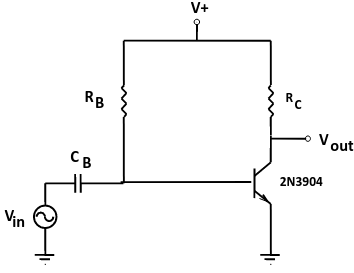
\includegraphics[width=.7\textwidth]{Figures/L4C1}
  \caption{Common Emitter Amplifier with: $R_B=309[\si{\kilo\ohm}]$, $R_C=1[\si{\kilo\ohm}]$, $C_B=1.5[\si{\micro\farad}]$, $V^+=10[\si{\volt}]$, and $V_{in}=10[\si{\milli\volt}_{0p}]$}
  \label{fig:1}
\end{figure}

Physically, this looked like:

\begin{figure}[H]
  \centering
  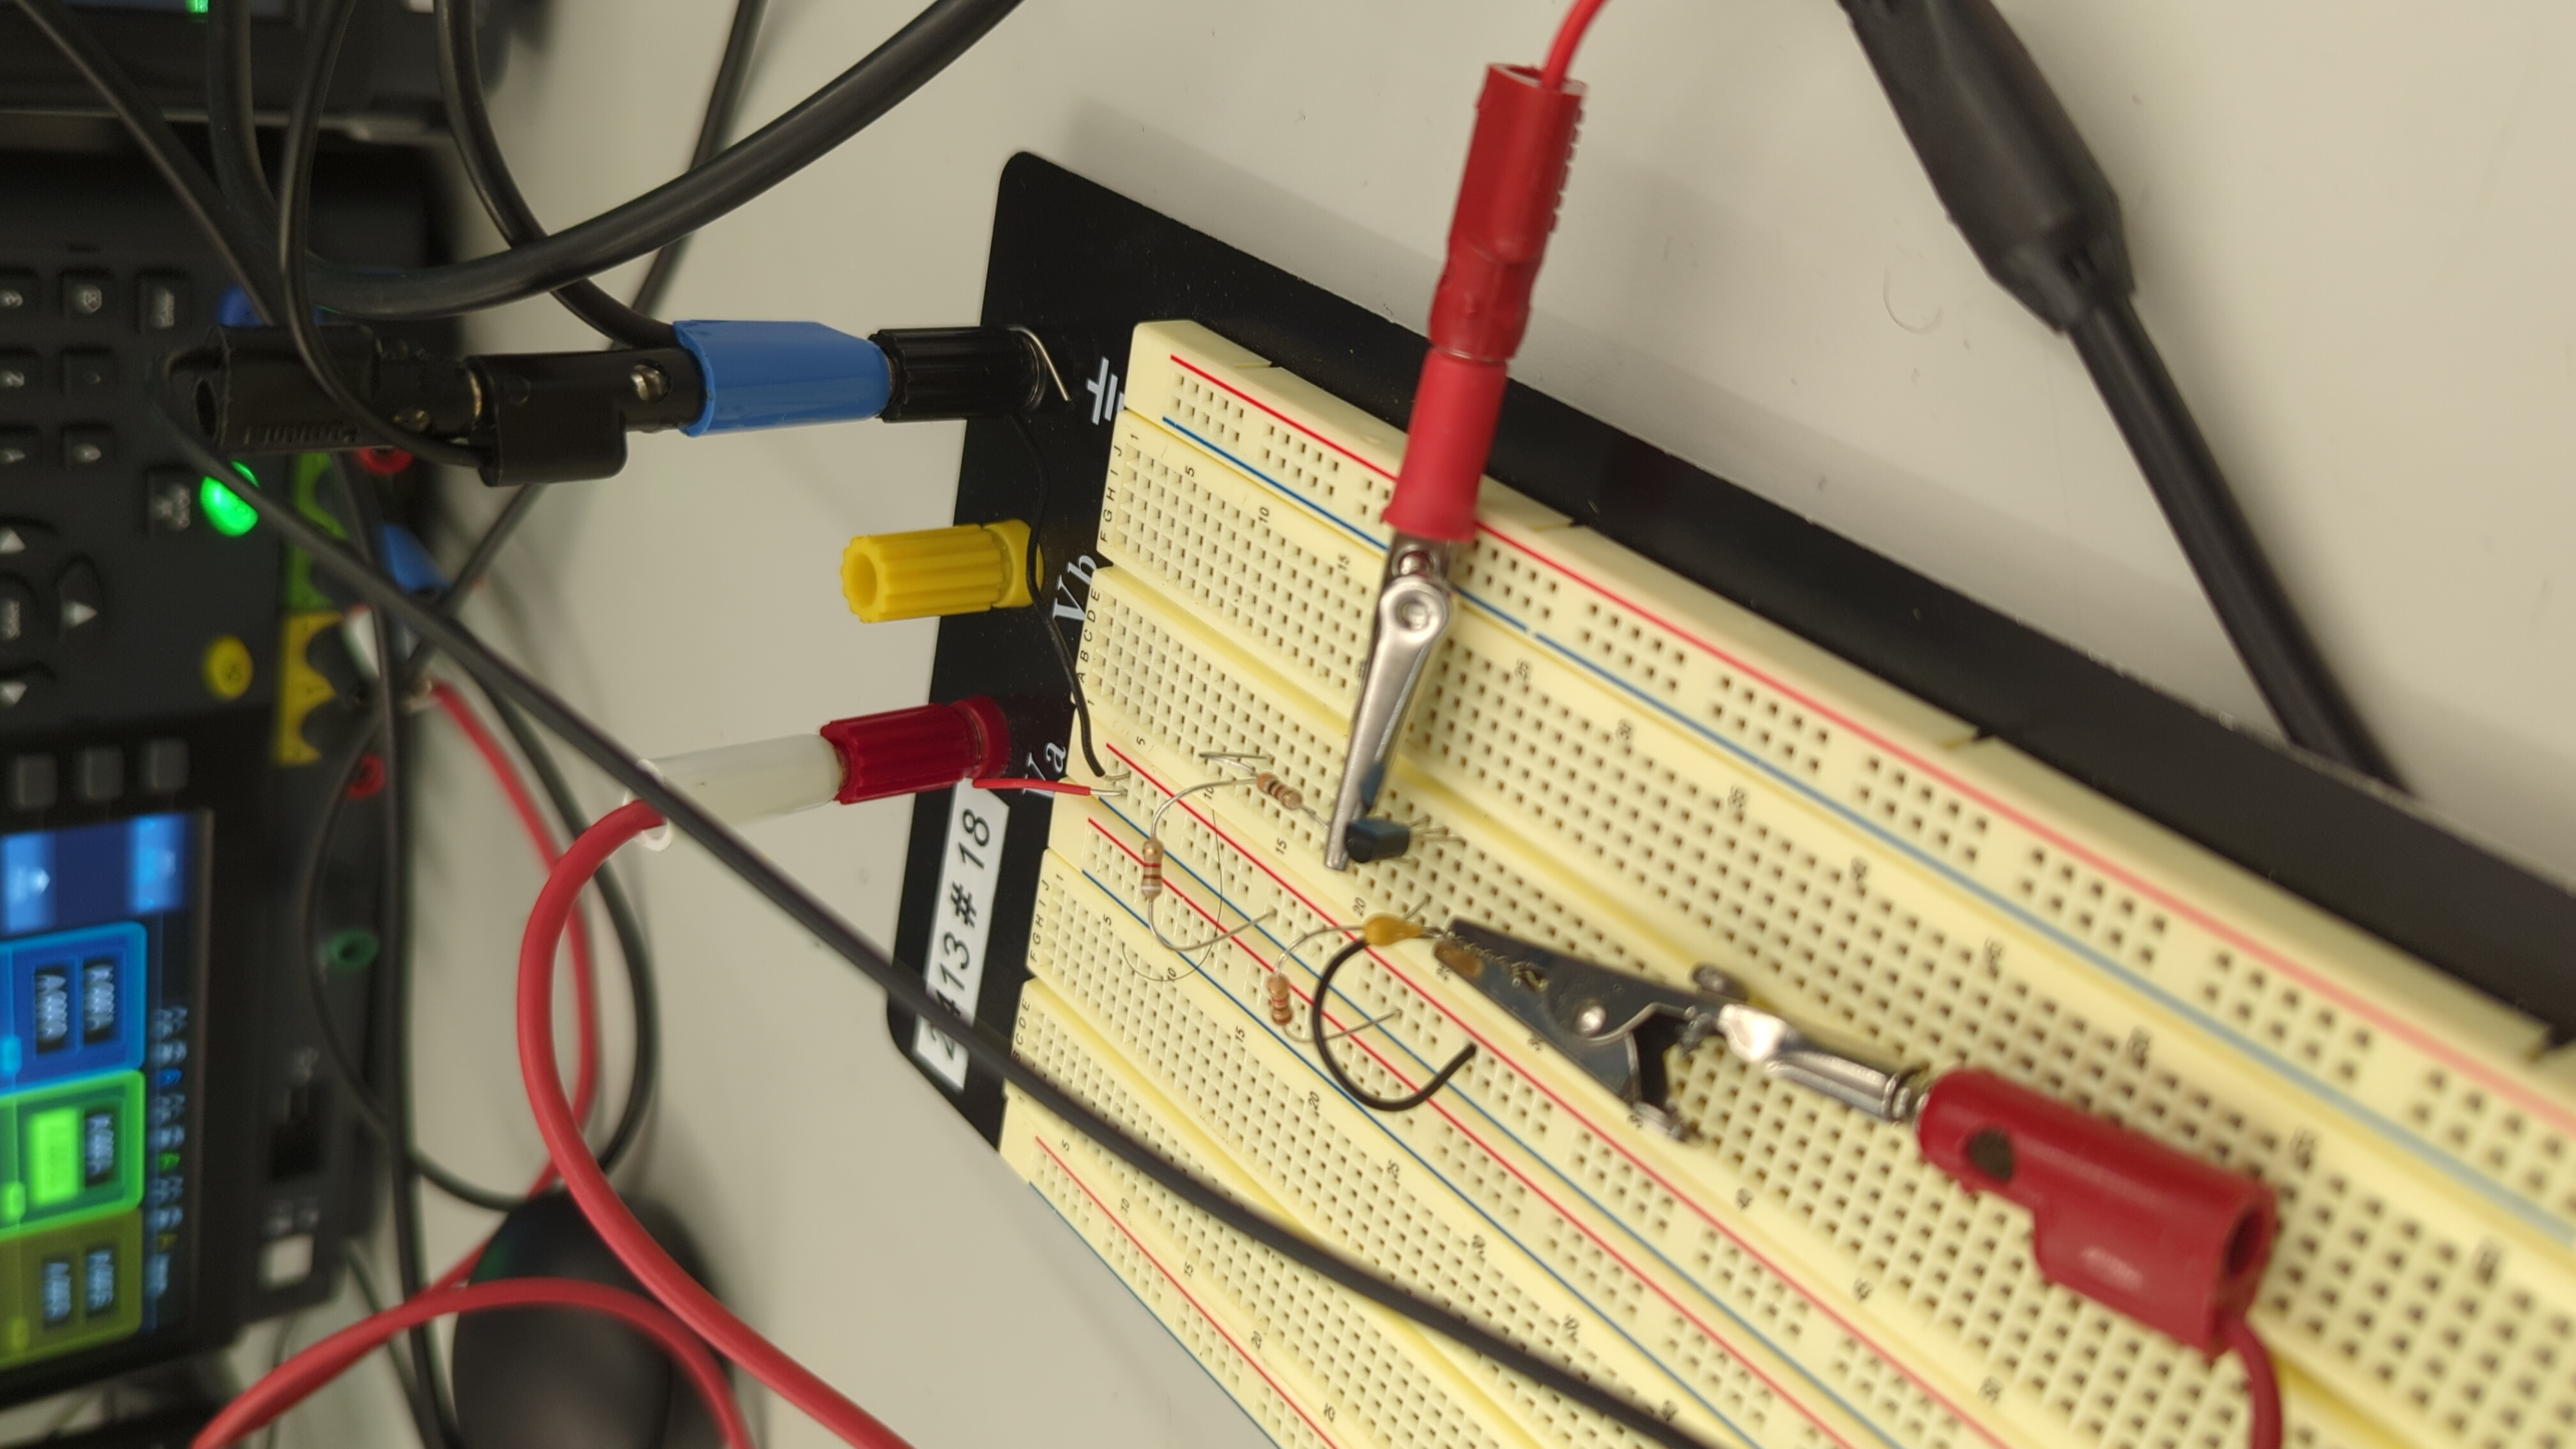
\includegraphics[width=.9\textwidth]{Figures/L4F1}
  \caption{Constructed Amplifier (Unstable)}
  \label{fig:2}
\end{figure}

\subsection{Confirming Active State}

Based on the parameters described in Figure \ref{fig:1}, we measure: $V_{CE}=2.75[\si{\volt}]$ and $V_{BE}=.715[\si{\volt}]$. Given that $V_{CE}>V_{BE}$, we conclude that the above amplifier is biased in the forward active region.

\subsection{Calculating Transconductance Gain}

We now calculate the collector current as:

$$I_C=\frac{V_{CE}-.7}{1k}$$
$$I_C=\frac{2.75-.7}{1k}$$
$$\boxed{I_C=2.05[\si{\milli\ampere}]}$$

Since we know that, at room temperature, $V_T=26[\si{\milli\ampere}]$, we may calculate:

$$g_m=\frac{2.05}{26}$$
$$\boxed{g_m=78.896[\si{\milli\siemen}]}$$

\subsection{Calculating the DC Gain ($\beta_{DC}$)}

We may experimentally determine the gain by finding:

$$I_B=\frac{.715-.7}{1k}$$
$$\boxed{I_B=15[\si{\micro\ampere}]}$$

Which gives us:

$$\beta_{DC}=\frac{I_C}{I_B}$$
$$\beta_{DC}=\frac{2.05}{.015}$$
$$\boxed{\beta_{DC}=136.67}$$

\subsection{Calculating $r_{\pi}$}

We may use our obtained values from above to find:

$$r_{\pi}=\frac{\beta}{g_m}$$
$$r_{\pi}=\frac{136.67}{.078846}$$
$$\boxed{r_{\pi}=1733.4[\si{\ohm}]}$$

\subsection{Calculating the Voltage Gain}

We may obtain the voltage gain using:

$$A_v=-g_mR_C$$
$$A_v=-(.078846)(1k)$$
$$\boxed{A_v=-78.846}$$

Note that the measured voltage gain was approximately $-80$, which is in line with the calculated gain.

\subsection{Experimentally Obtaining Voltage Gain}

Measuring the input voltage, we find that, zero-to-peak, it is a nominal $7[\si{\milli\volt}]$, while the output was $560[\si{\milli\volt}]$, and phase shifted by 180$^{\circ}$. This gives us an experimental gain of:

$$A_v=\frac{-560}{7}$$
$$\boxed{A_v=-80}$$

When $r_b=200[\si{\ohm}]$, the voltage gain meets a slight division, which gives us:

$$A_v=-g_m\left( \frac{r_{\pi}}{r_b+r_{\pi}} \right)$$
$$A_v=-(.78846)\left( \frac{1733.4}{200+1733.4} \right)$$
$$\boxed{A_v=-70.69}$$

We may observe that, in such a case, the voltage gain is slightly reduced.

\subsection{Output Clipping}

Experimentally, we observe clipping at $.15[\si{\volt}]$ and $0[\si{\volt}]$. We may explain the minimum because there is no negative voltage swing with the BJT. In the other hand, there is a maximum because the voltage gain times $.15[\si{\volt}]$ is greater than the supply voltage (as experienced with operational amplifiers).

\subsubsection{Gain Sensitivity to Supply Voltage}

Changing the supply voltage to $8[\si{\volt}]$, we see the voltage gain become:

$$A_v=-\frac{4.8}{.053}$$
$$\boxed{A_v=-90.566}$$

Changing the input to the $12[\si{\volt}]$, we see the gain magnitude increases to:

$$A_v=-\frac{5.6}{.047}$$
$$\boxed{A_v=-119.15}$$

We may determine that the amplifier is sensitive to changes in the supply voltage because the collector current depends on the collector-to-emitter voltage, and the collector-to-emitter voltage, in turn, depends on the supply voltage. Because the transconductance gain of the amplifier depends on the collector current, a change in the collector-to-emitter voltage results in a change in the gain, which depends on the transconductance gain.

\subsection{Frequency Response of the Gain}

We may observe that the upper corner frequency occurs at, approximately, $f_{crit}=730[\si{\kilo\hertz}]$. On the other hand, the lower corner frequency occurs at, approximately, $f_{crit}=14[\si{\kilo\hertz}]$. According to these values, though not ideal, this amplifier is best suited for an AM Radio. It can operate at a lower frequency by using a different capacitor value, which we observed by increasing the capacitance value.

\subsection{Stabilizing the Amplifier}

After introducing the changes to the amplifier, we see that the voltage gain is:

$$A_v=-4.7$$

and, thus, it is insensitive to changes in $V^+$. As expected, the gain decreased. Calculating the gain, we find that $A_v=-4$, which is just a bit lesser in magnitude than the value above. Introducing refrigerant increased the magnitude of the gain to $A_v=-21$, with the peak-to-peak output voltage going from $8.2\to8[\si{\volt}]$, and the input voltage remaining at $.44[\si{\volt}]$

\subsection{Constructing A Stable Amplifier}

With values derived in the pre-lab, we construct a stable amplifier as follows:

\begin{figure}[H]
  \centering
  \tikzset{every picture/.style={line width=0.75pt}} %set default line width to 0.75pt        

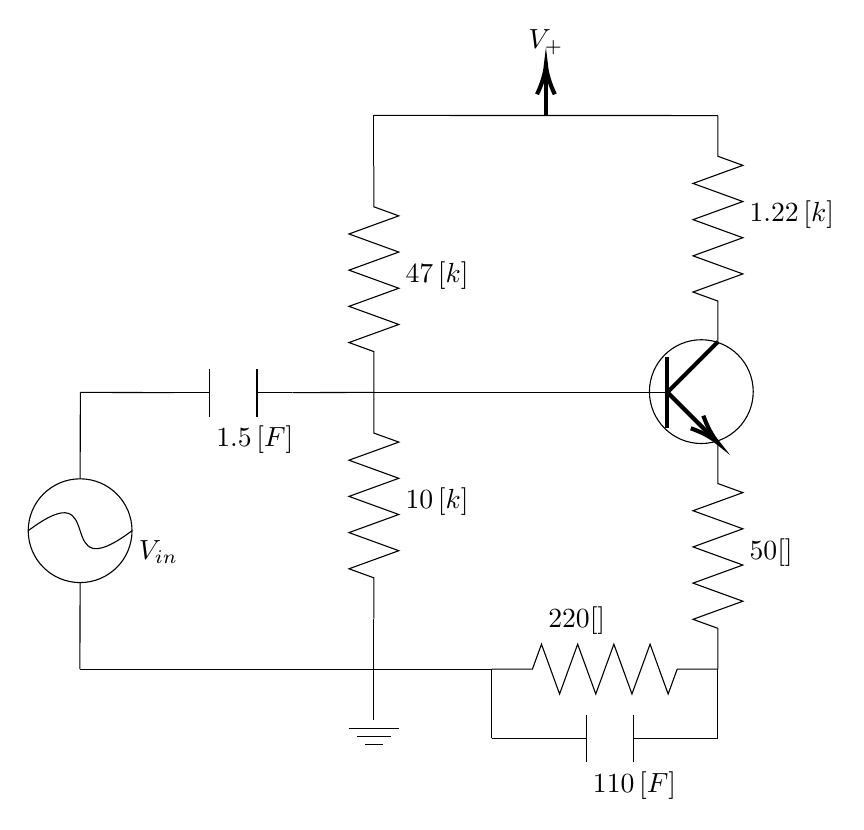
\begin{tikzpicture}[x=0.75pt,y=0.75pt,yscale=-1,xscale=1]
%uncomment if require: \path (0,590); %set diagram left start at 0, and has height of 590

%Shape: Resistor [id:dp3833220318083407] 
\draw   (365,122) -- (365,141.62) -- (377,145.98) -- (353,154.7) -- (377,163.42) -- (353,172.14) -- (377,180.86) -- (353,189.58) -- (377,198.3) -- (353,207.02) -- (365,211.38) -- (365,231) ;
%Shape: Resistor [id:dp8587716412218651] 
\draw   (365,279.68) -- (365,299.3) -- (377,303.66) -- (353,312.38) -- (377,321.1) -- (353,329.82) -- (377,338.54) -- (353,347.26) -- (377,355.98) -- (353,364.7) -- (365,369.06) -- (365,388.68) ;
%Straight Lines [id:da4792550547478952] 
\draw [line width=1.5]    (365,231) -- (340.66,255.34) ;
%Straight Lines [id:da7608141958592706] 
\draw [line width=1.5]    (362.88,277.56) -- (340.66,255.34) ;
\draw [shift={(365,279.68)}, rotate = 225] [color={rgb, 255:red, 0; green, 0; blue, 0 }  ][line width=1.5]    (14.21,-4.28) .. controls (9.04,-1.82) and (4.3,-0.39) .. (0,0) .. controls (4.3,0.39) and (9.04,1.82) .. (14.21,4.28)   ;
%Straight Lines [id:da17503758559340787] 
\draw [line width=1.5]    (340.66,272.55) -- (340.66,238.13) ;
%Shape: Circle [id:dp10180694146995228] 
\draw   (332,255) .. controls (332,241.19) and (343.19,230) .. (357,230) .. controls (370.81,230) and (382,241.19) .. (382,255) .. controls (382,268.81) and (370.81,280) .. (357,280) .. controls (343.19,280) and (332,268.81) .. (332,255) -- cycle ;
%Straight Lines [id:da49812635295344454] 
\draw    (340.66,255.34) -- (199.24,255.34) ;
%Shape: Resistor [id:dp2521464987894332] 
\draw   (256,388.68) -- (275.62,388.68) -- (279.98,376.68) -- (288.7,400.68) -- (297.42,376.68) -- (306.14,400.68) -- (314.86,376.68) -- (323.58,400.68) -- (332.3,376.68) -- (341.02,400.68) -- (345.38,388.68) -- (365,388.68) ;
%Shape: Resistor [id:dp49592375364034] 
\draw   (199.24,255.34) -- (199.24,274.96) -- (211.24,279.32) -- (187.24,288.04) -- (211.24,296.76) -- (187.24,305.48) -- (211.24,314.2) -- (187.24,322.92) -- (211.24,331.64) -- (187.24,340.36) -- (199.24,344.72) -- (199.24,364.34) ;
%Shape: Resistor [id:dp3891387019727379] 
\draw   (199.24,146.34) -- (199.24,165.96) -- (211.24,170.32) -- (187.24,179.04) -- (211.24,187.76) -- (187.24,196.48) -- (211.24,205.2) -- (187.24,213.92) -- (211.24,222.64) -- (187.24,231.36) -- (199.24,235.72) -- (199.24,255.34) ;
%Shape: Circle [id:dp415368708502455] 
\draw   (32.7,322.01) .. controls (32.7,308.2) and (43.89,297.01) .. (57.7,297.01) .. controls (71.51,297.01) and (82.7,308.2) .. (82.7,322.01) .. controls (82.7,335.82) and (71.51,347.01) .. (57.7,347.01) .. controls (43.89,347.01) and (32.7,335.82) .. (32.7,322.01) -- cycle ;
%Straight Lines [id:da3349770798972058] 
\draw    (103,255.5) -- (57.82,255.34) ;
%Straight Lines [id:da43907617946532207] 
\draw    (256,388.68) -- (57.58,388.68) ;
%Straight Lines [id:da13936423966023304] 
\draw    (199.24,388.76) -- (199.24,364.34) ;
%Straight Lines [id:da34855689912084087] 
\draw    (57.7,297.01) -- (57.82,255.34) ;
%Straight Lines [id:da7839594312474344] 
\draw    (57.58,388.68) -- (57.7,347.01) ;
%Curve Lines [id:da13958765371739967] 
\draw    (32.7,322.01) .. controls (72.7,292.01) and (42.7,352.01) .. (82.7,322.01) ;
%Shape: Contact [id:dp174874215762453] 
\draw   (103,255.5) -- (120.1,255.5) (160,255.5) -- (142.9,255.5) (120.1,244) -- (120.1,267) (142.9,244) -- (142.9,267) ;
%Straight Lines [id:da3250650556708795] 
\draw    (199.24,255.34) -- (160,255.5) ;
%Shape: Contact [id:dp955820902288611] 
\draw   (284.42,422.1) -- (301.52,422.1) (341.42,422.1) -- (324.32,422.1) (301.52,410.6) -- (301.52,433.6) (324.32,410.6) -- (324.32,433.6) ;
%Straight Lines [id:da8839082103913728] 
\draw    (365,422.1) -- (365,388.68) ;
%Straight Lines [id:da4288509553556663] 
\draw    (256,422.1) -- (256,388.68) ;
%Straight Lines [id:da7017573981053074] 
\draw    (256,422.1) -- (272.71,422.1) -- (284.42,422.1) ;
%Straight Lines [id:da2830731599338929] 
\draw    (341.42,422.1) -- (353.29,422.1) -- (365,422.1) ;
%Straight Lines [id:da9688326739052082] 
\draw    (365,122) -- (199.24,121.92) ;
%Straight Lines [id:da8636007395671251] 
\draw    (199.24,146.34) -- (199.24,121.92) ;
%Straight Lines [id:da18324498073500228] 
\draw    (199.24,413.18) -- (199.24,388.76) ;
%Straight Lines [id:da061393554026757724] 
\draw    (187.03,417.18) -- (211.45,417.18) ;
%Straight Lines [id:da9729158195349732] 
\draw    (191.03,421.18) -- (207.45,421.18) ;
%Straight Lines [id:da008040790617349192] 
\draw    (195.03,425.18) -- (203.45,425.18) ;
%Straight Lines [id:da7717989098960579] 
\draw [line width=1.5]    (282.12,121.96) -- (282.12,100.54) ;
\draw [shift={(282.12,97.54)}, rotate = 90] [color={rgb, 255:red, 0; green, 0; blue, 0 }  ][line width=1.5]    (14.21,-4.28) .. controls (9.04,-1.82) and (4.3,-0.39) .. (0,0) .. controls (4.3,0.39) and (9.04,1.82) .. (14.21,4.28)   ;

% Text Node
\draw (84.7,325.41) node [anchor=north west][inner sep=0.75pt]    {$V_{in}$};
% Text Node
\draw (282.12,94.14) node [anchor=south] [inner sep=0.75pt]    {$V_{+}$};
% Text Node
\draw (122.1,270.4) node [anchor=north west][inner sep=0.75pt]    {$1.5\left[ \Micro \text{F}\right]$};
% Text Node
\draw (303.52,437) node [anchor=north west][inner sep=0.75pt]    {$110\left[ \Micro \text{F}\right]$};
% Text Node
\draw (213.24,300.16) node [anchor=north west][inner sep=0.75pt]    {$10\left[\text{k} \si{\ohm}\right]$};
% Text Node
\draw (379,324.5) node [anchor=north west][inner sep=0.75pt]    {$50[ \si{\ohm}]$};
% Text Node
\draw (281.98,373.28) node [anchor=south west] [inner sep=0.75pt]    {$220[ \si{\ohm}]$};
% Text Node
\draw (379,177.46) node [anchor=south west] [inner sep=0.75pt]    {$1.22\left[\text{k} \si{\ohm}\right]$};
% Text Node
\draw (213.24,191.16) node [anchor=north west][inner sep=0.75pt]    {$47\left[\text{k} \si{\ohm}\right]$};


\end{tikzpicture}

  \caption{Stable BJT Amplifier}
  \label{fig:3}
\end{figure}

Physically, the circuit was constructed as shown below:

\begin{figure}[H]
  \centering
  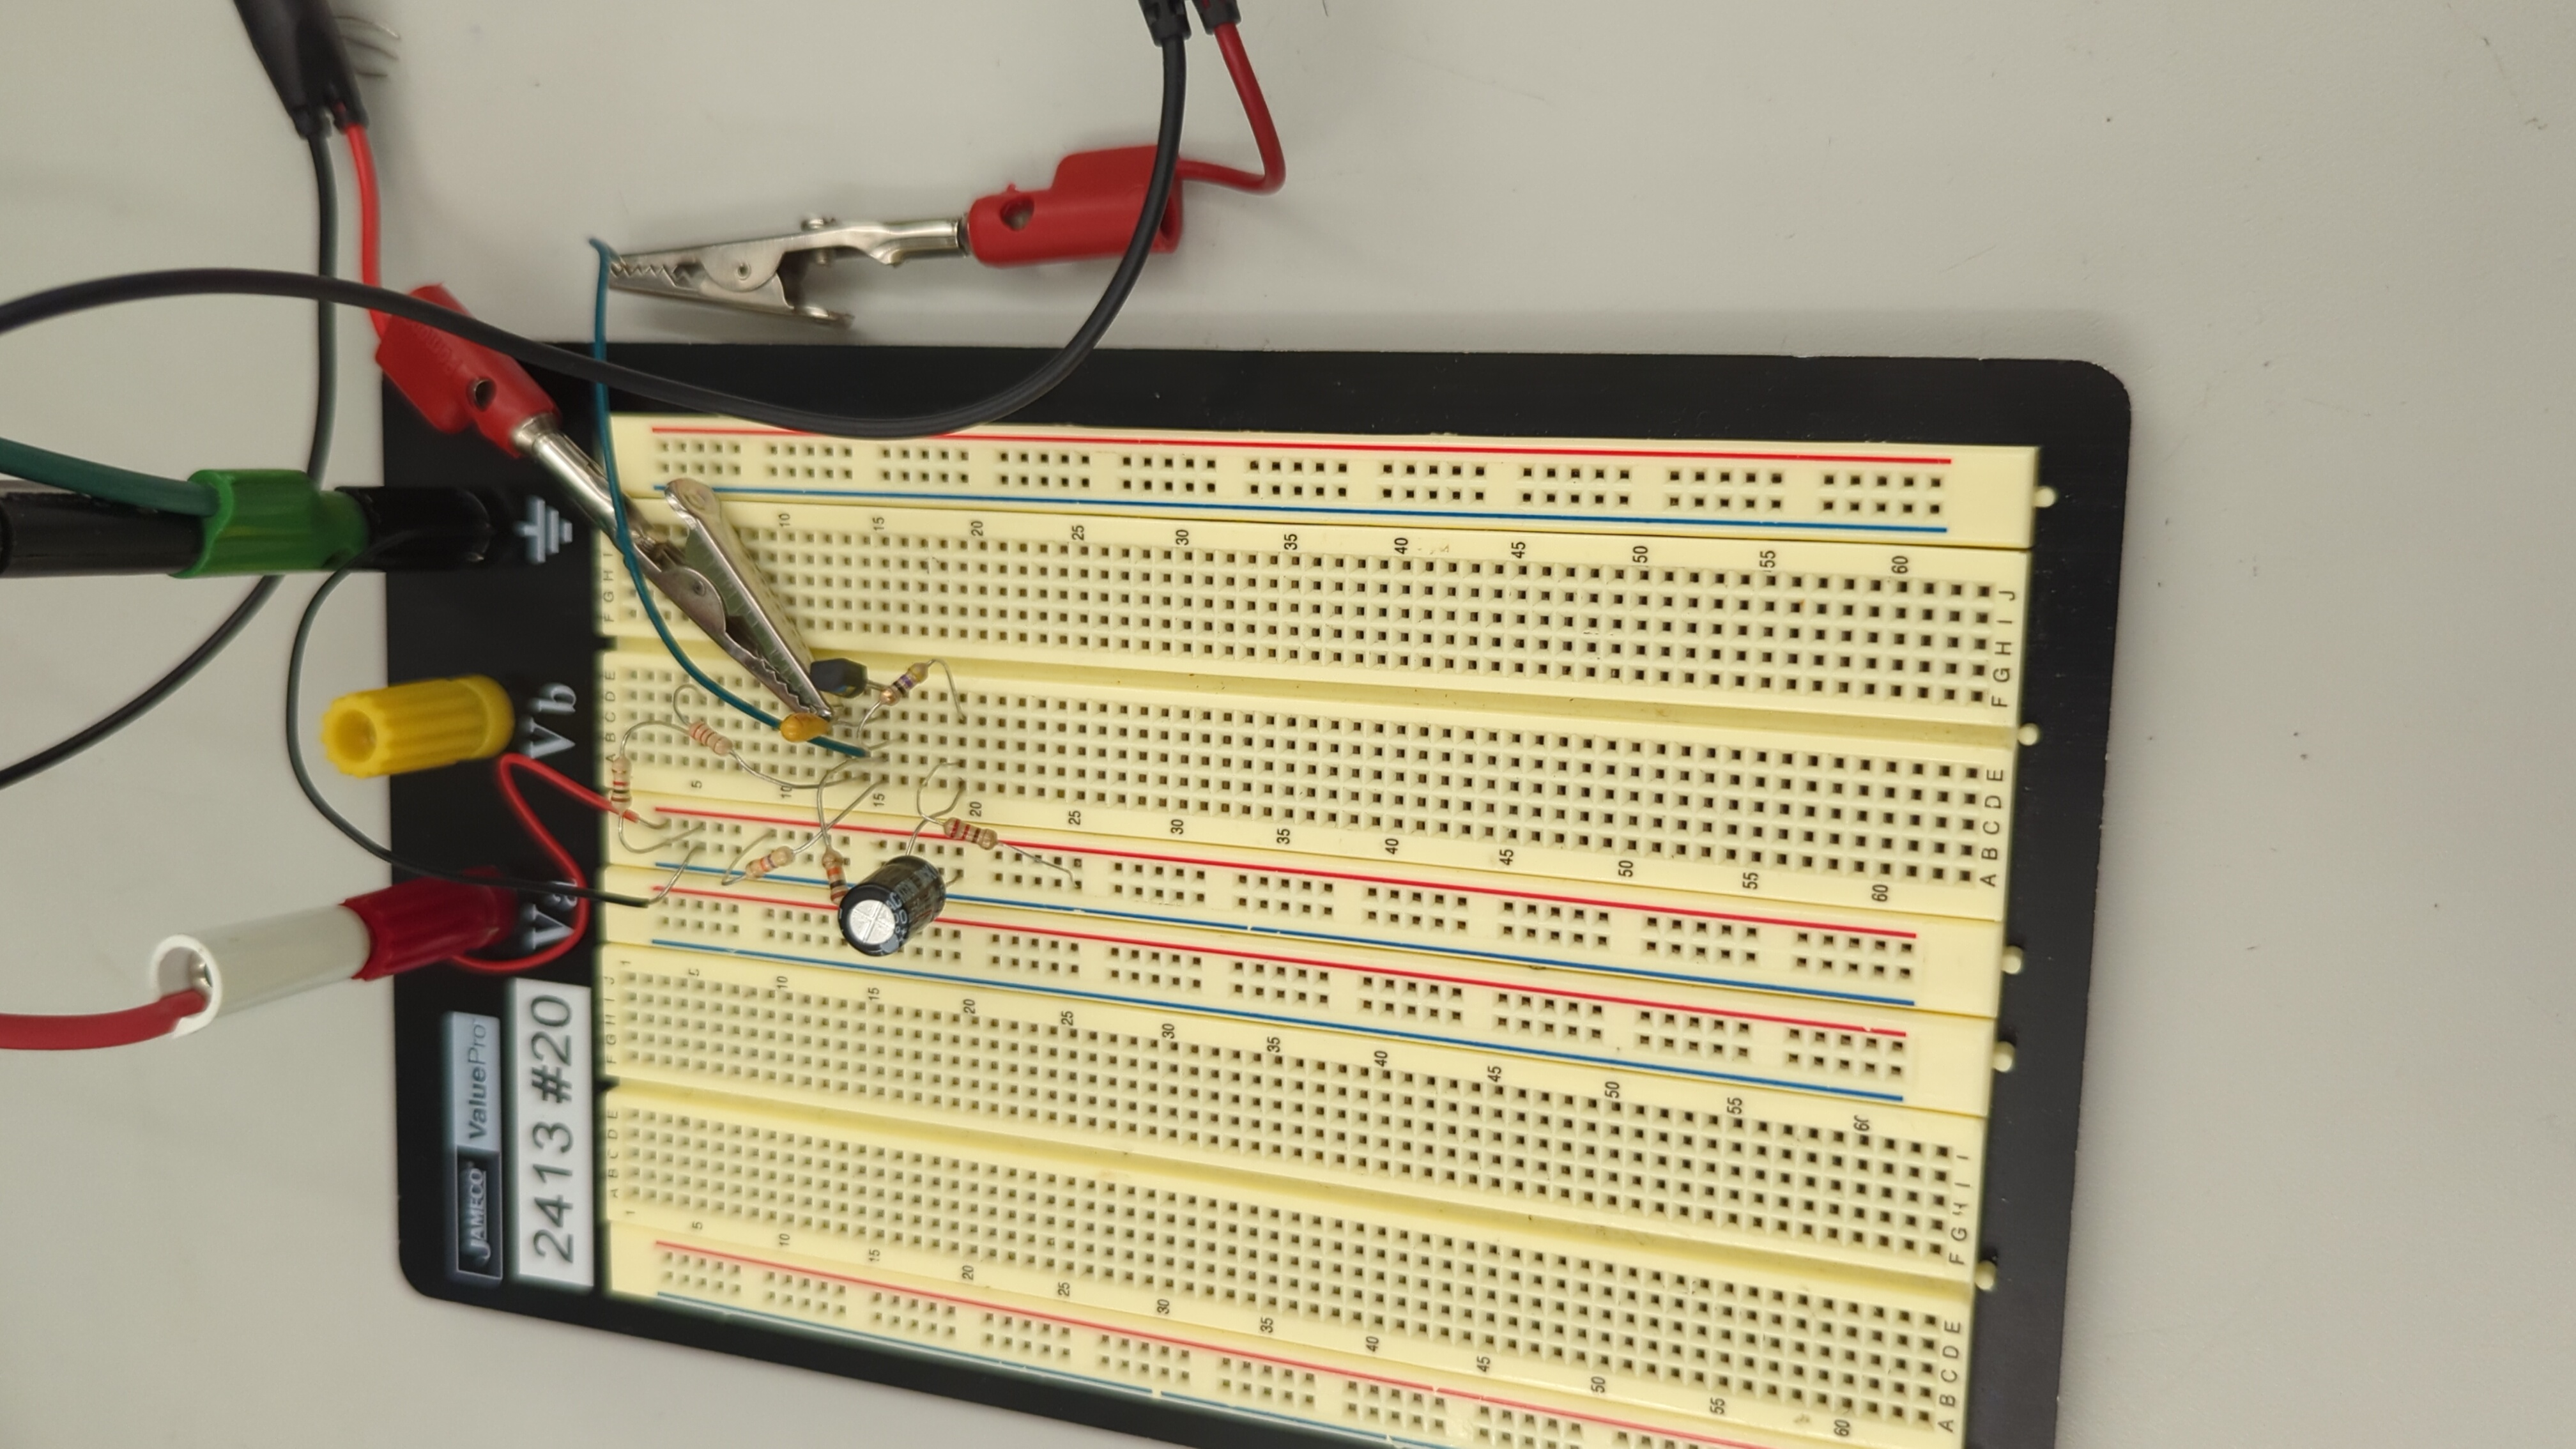
\includegraphics[width=.9\textwidth]{Figures/L4F2}
  \caption{Constructed Amplifier}
  \label{fig:4}
\end{figure}

The output for $V^{+}=8,10,$ and $12[\si{\volt}]$ is shown in Figures \ref{fig:5}-\ref{fig:7}:

\begin{figure}[H]
  \centering
  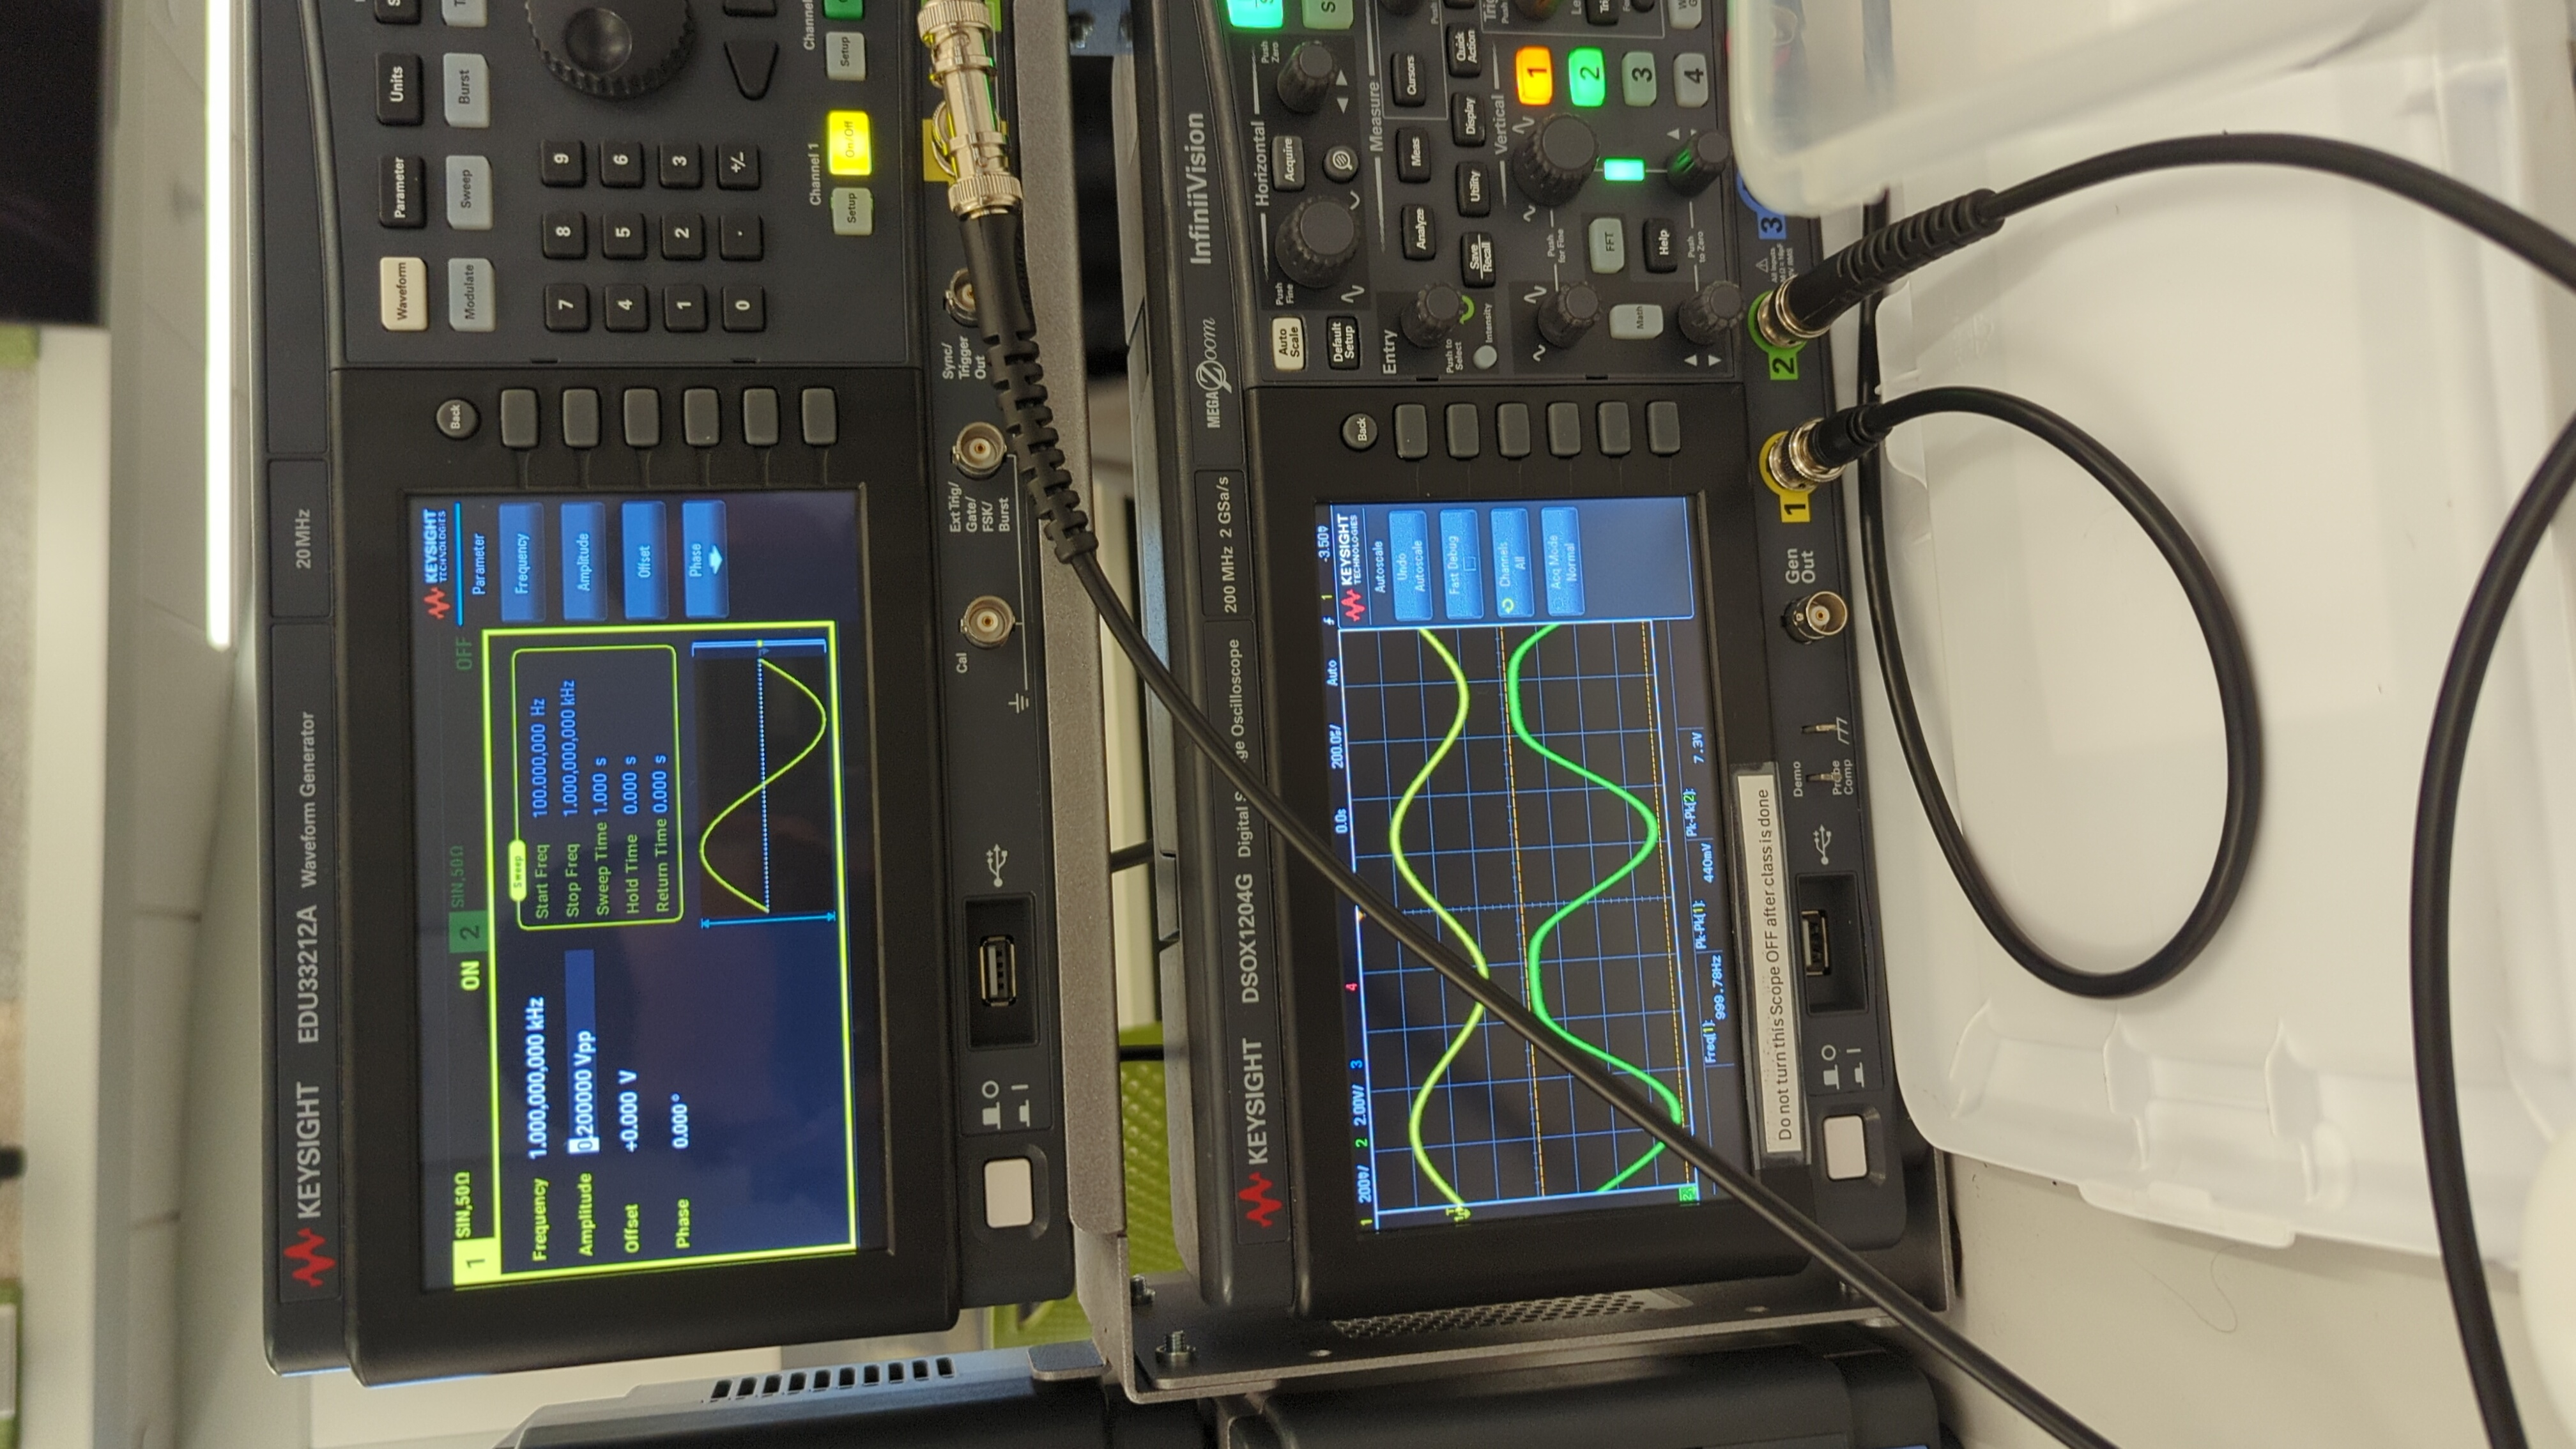
\includegraphics[width=.9\textwidth]{Figures/L4F3}
  \caption{Stable Amplifier, $V^{+}=8[\si{\volt}]$}
  \label{fig:5}
\end{figure}

\begin{figure}[H]
  \centering
  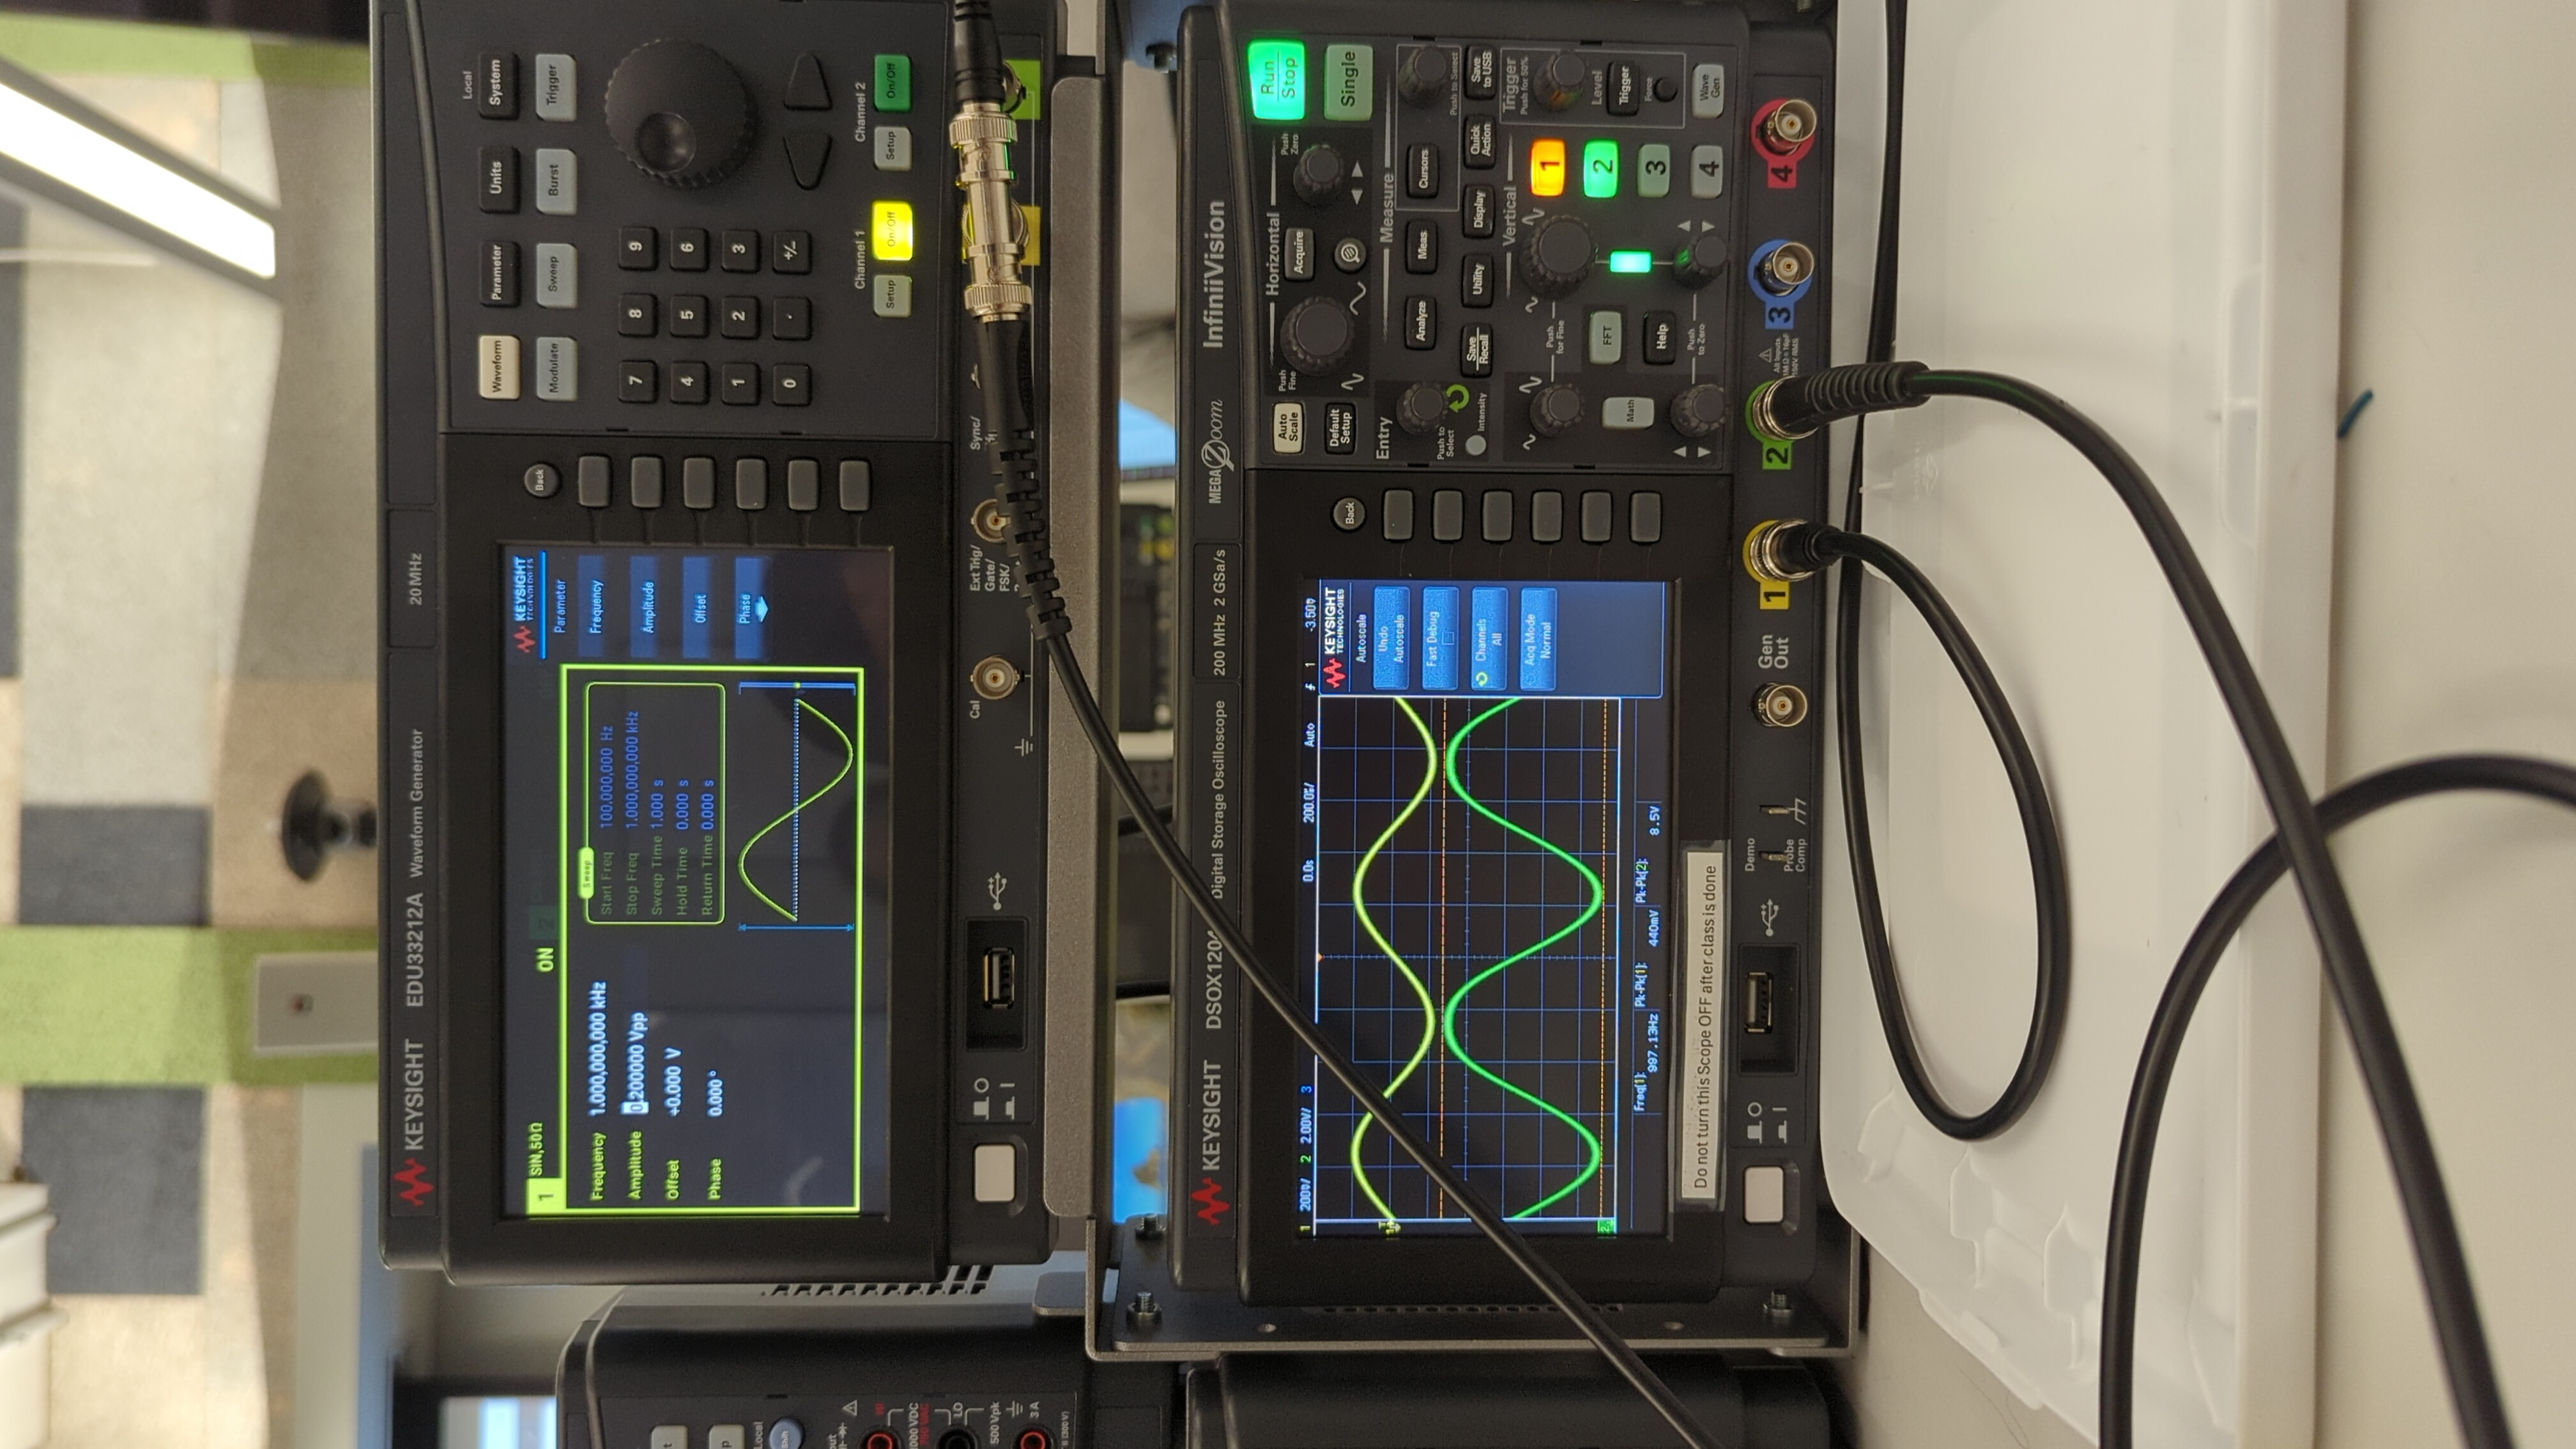
\includegraphics[width=.9\textwidth]{Figures/L4F4}
  \caption{Stable Amplifier, $V^{+}=10[\si{\volt}]$}
  \label{fig:6}
\end{figure}

\begin{figure}[H]
  \centering
  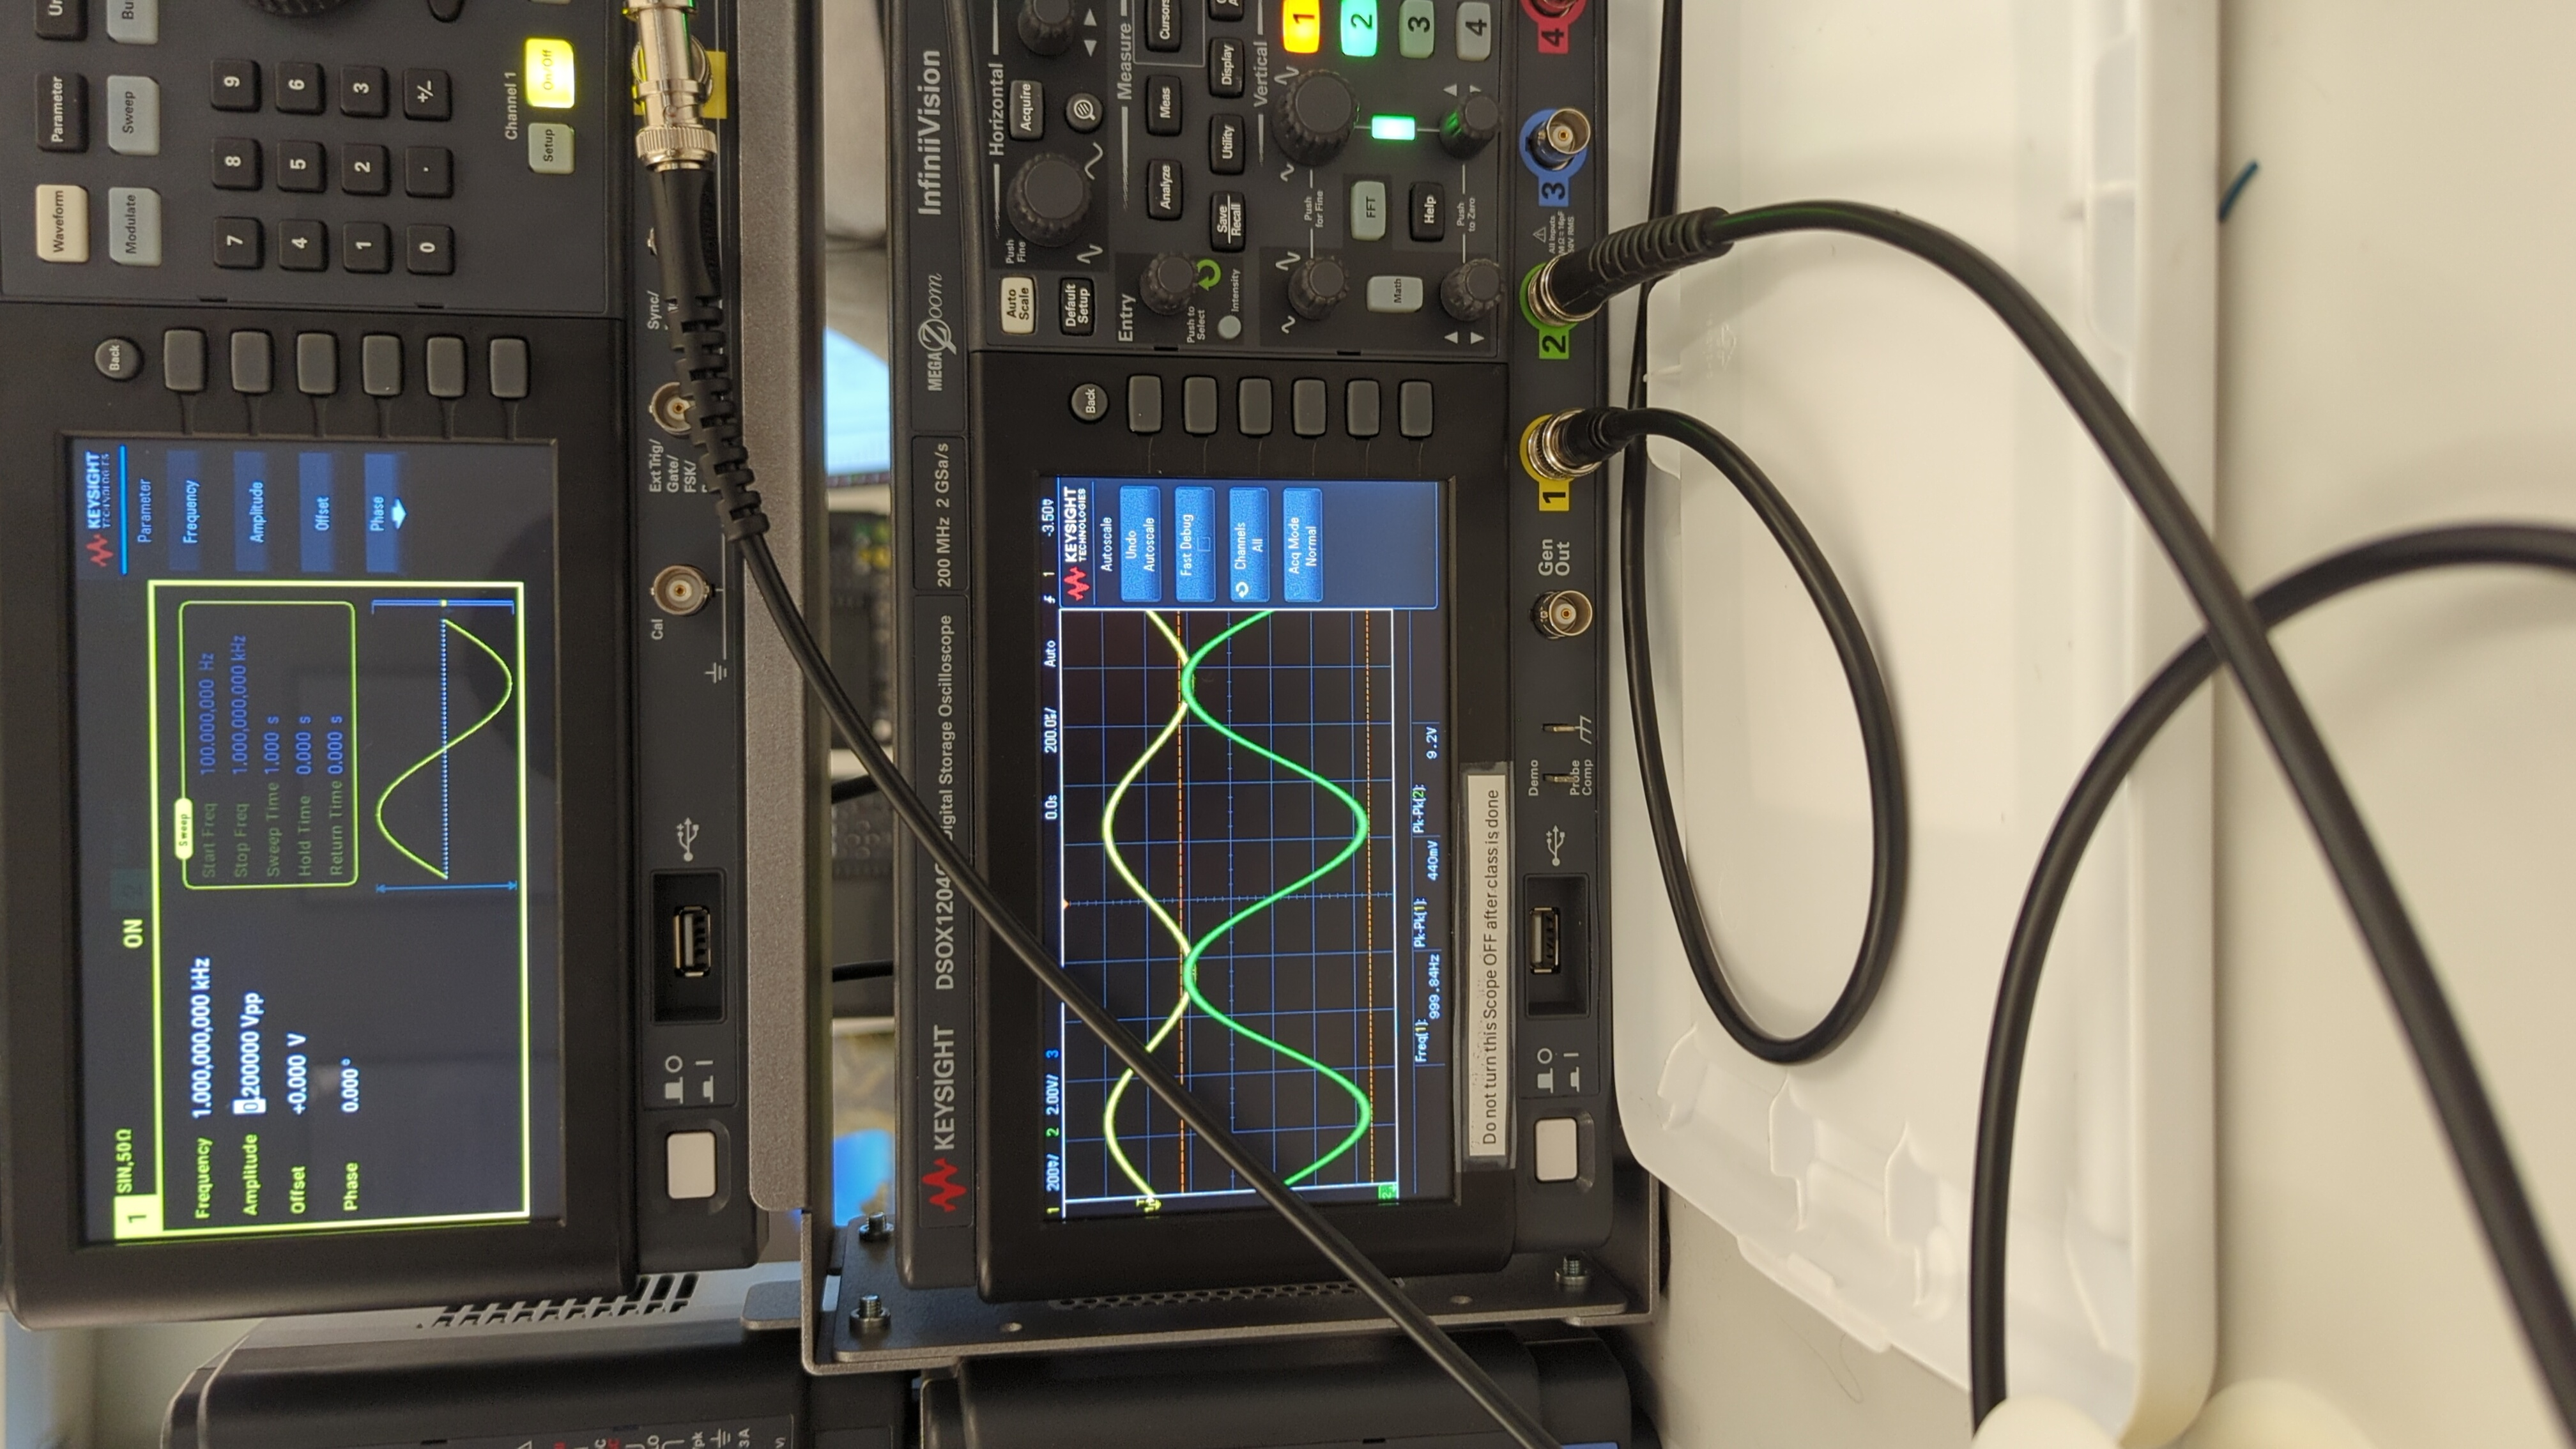
\includegraphics[width=.9\textwidth]{Figures/L4F5}
  \caption{Stable Amplifier, $V^{+}=12[\si{\volt}]$}
  \label{fig:7}
\end{figure}

We may see that, though at a lower supply voltage there is slight clipping (which is to be expected), the amplifier meets the performance requirements.

\subsection{Virtual Simulation}

\subsubsection{Part 1}

We simulate the following circuit:

\begin{figure}[H]
  \centering
  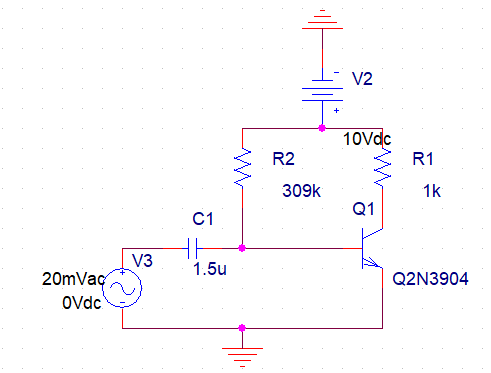
\includegraphics[width=.8\textwidth]{Figures/L4F6}
  \caption{Part 1, Initial Circuit Schematic}
  \label{fig:8}
\end{figure}

This produces the following responses:

\begin{figure}[H]
  \centering
  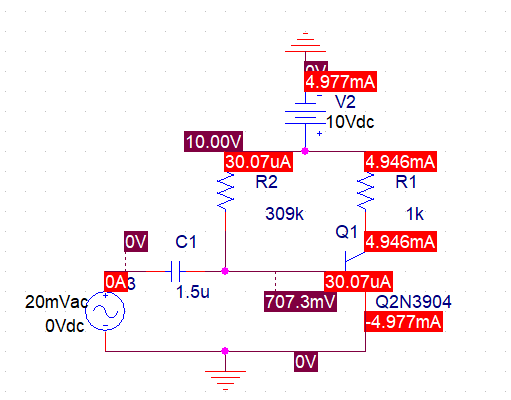
\includegraphics[width=.8\textwidth]{Figures/L4F7}
  \caption{Part 1, DC Response}
  \label{fig:9}
\end{figure}

\begin{figure}[H]
  \centering
  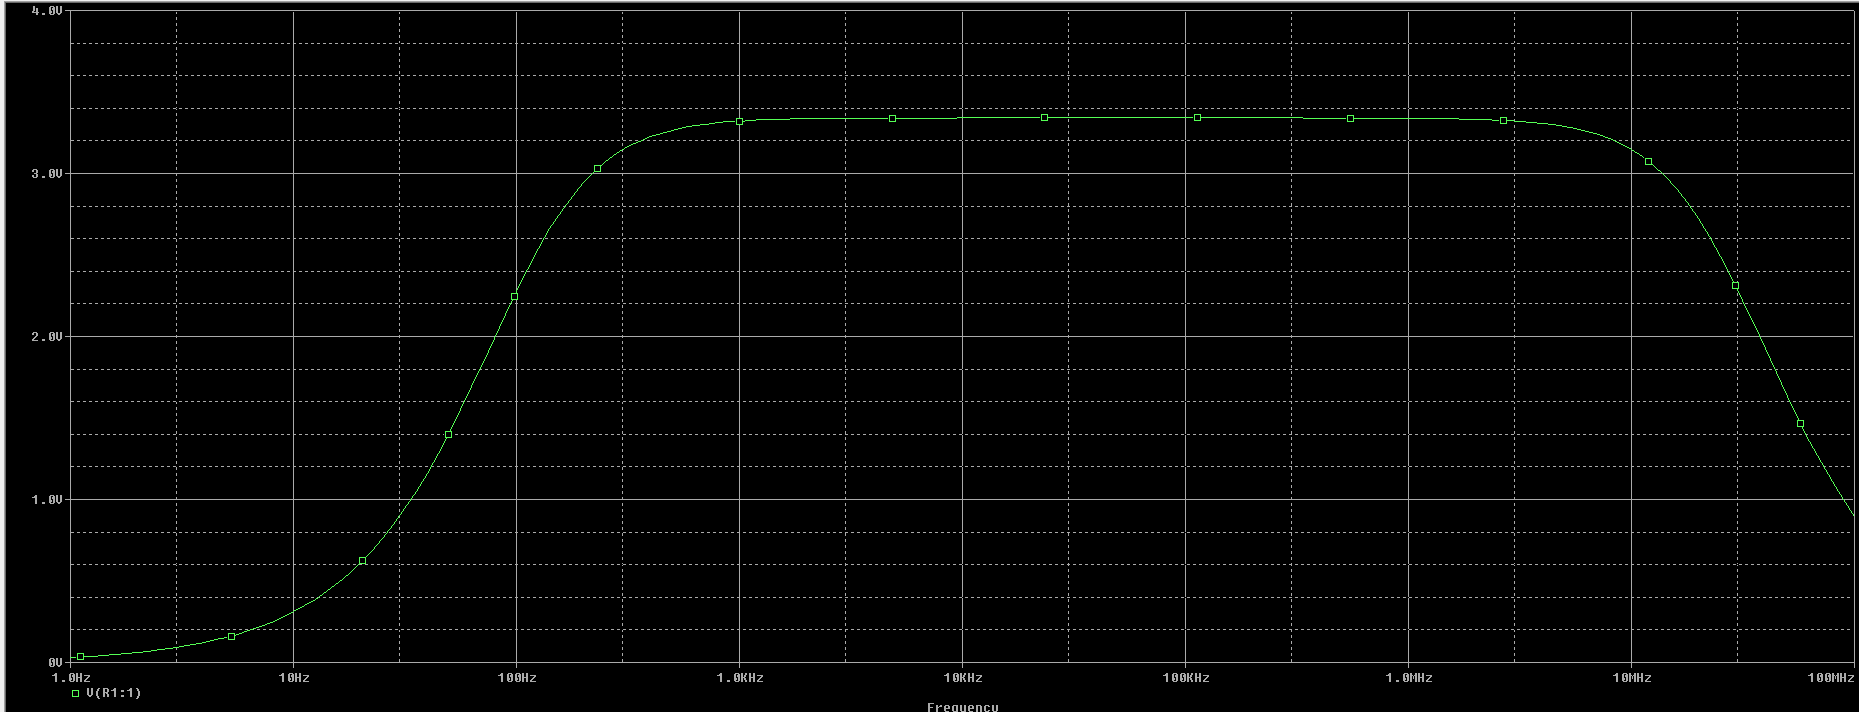
\includegraphics[width=.8\textwidth]{Figures/L4F8}
  \caption{Part 1, AC Response}
  \label{fig:10}
\end{figure}

Notice the corner frequencies and bandwidth in the plot above. We can then observe voltage clipping:

\begin{figure}[H]
  \centering
  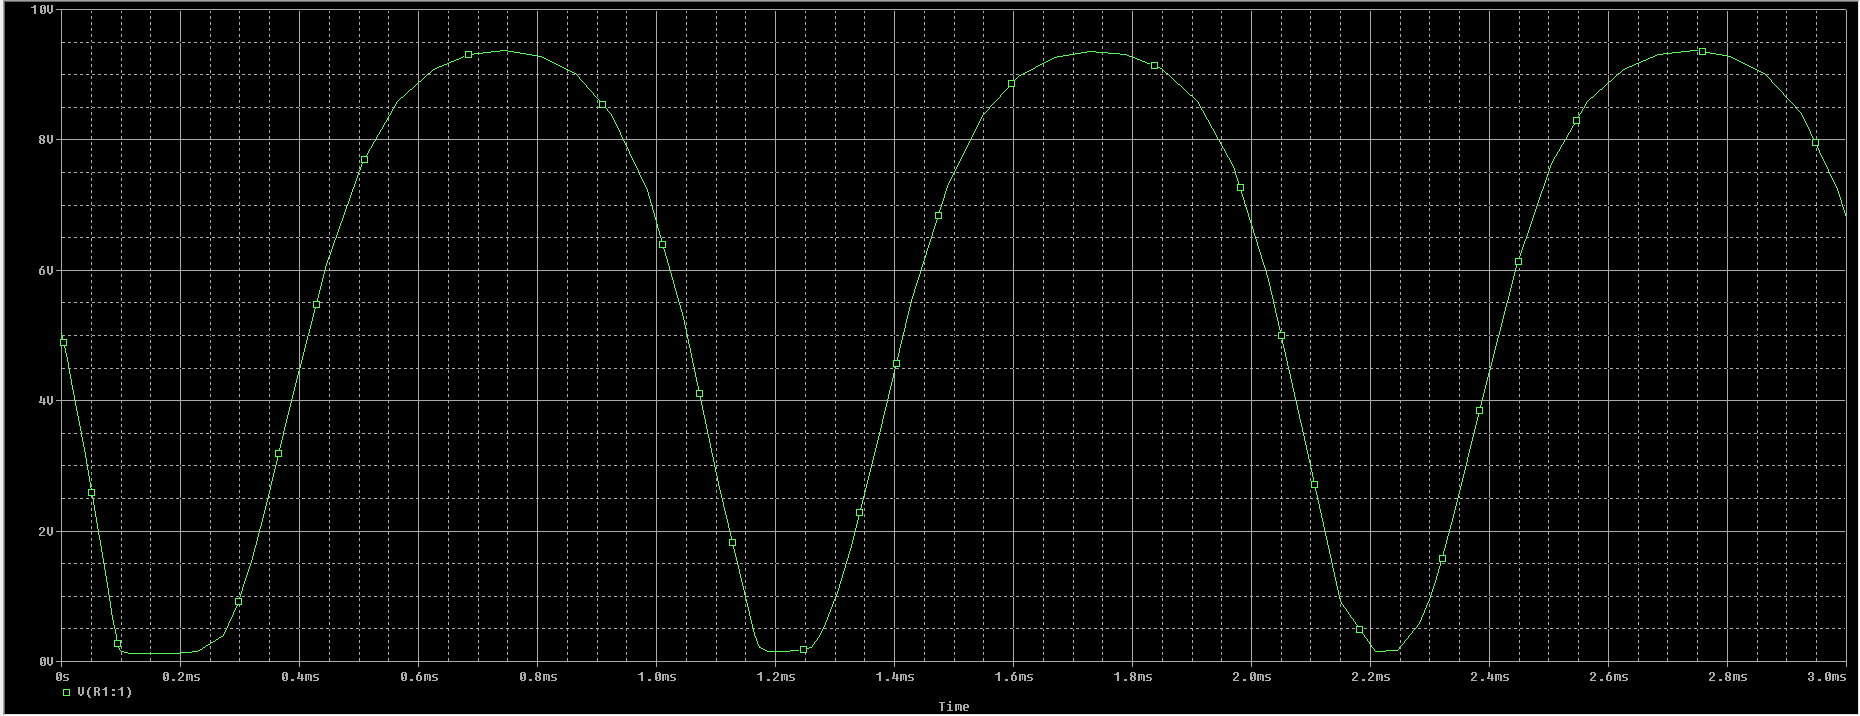
\includegraphics[width=.8\textwidth]{Figures/L4F9}
  \caption{Part 1, Clipping at just Above $.15[\si{\volt}_{0p}]$}
  \label{fig:11}
\end{figure}

The values agree with those measured and calculated. We now proceed to check the influence of the supply voltage:

\begin{figure}[H]
  \centering
  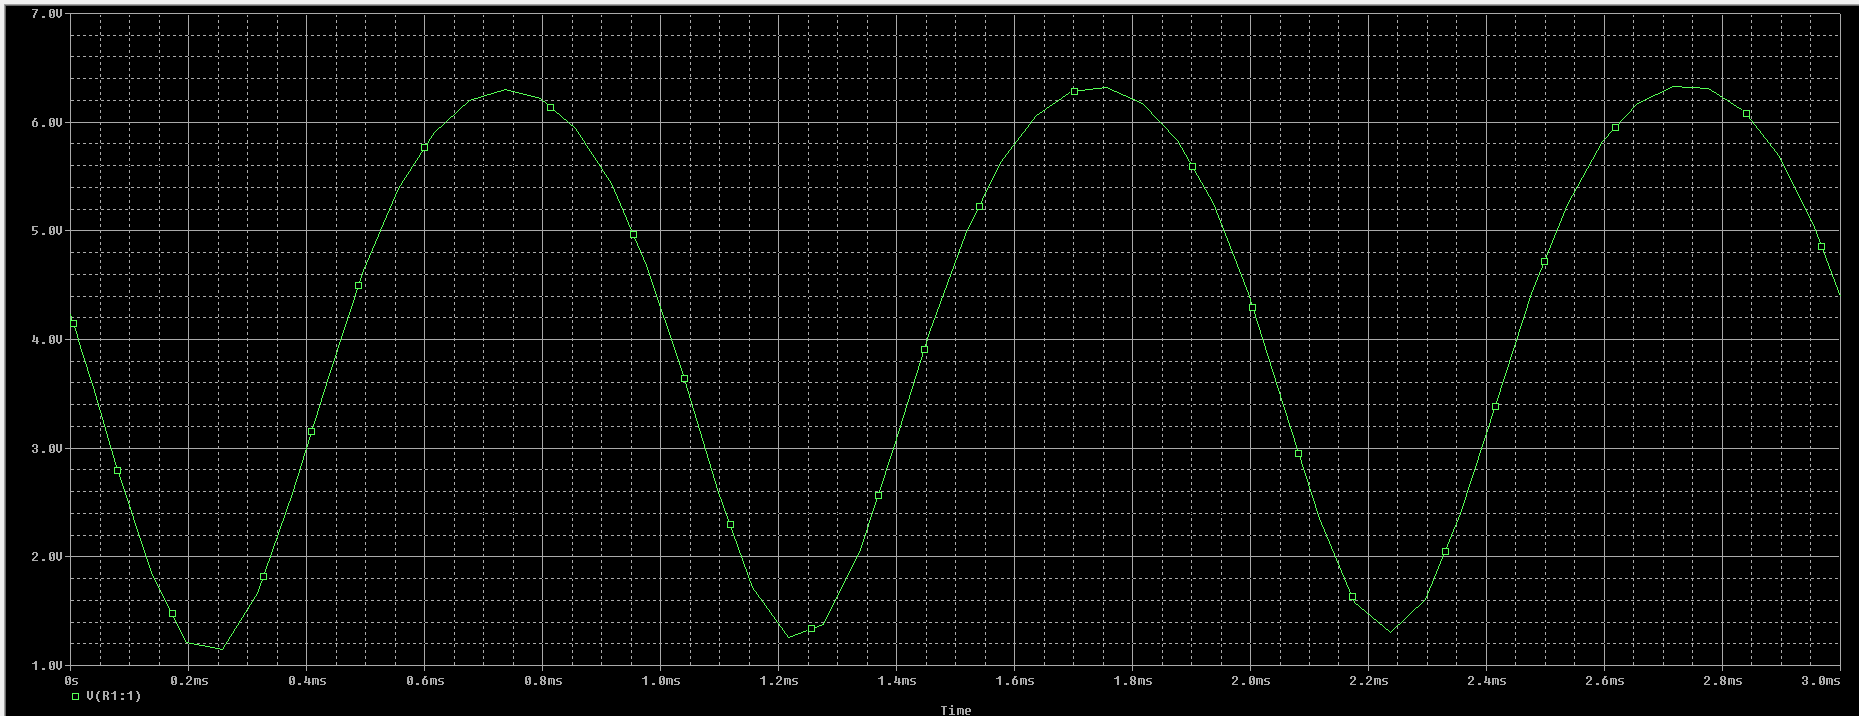
\includegraphics[width=.8\textwidth]{Figures/L4F10}
  \caption{Part 1, $8[\si{\volt}]$ Supply Voltage}
  \label{fig:12}
\end{figure}

\begin{figure}[H]
  \centering
  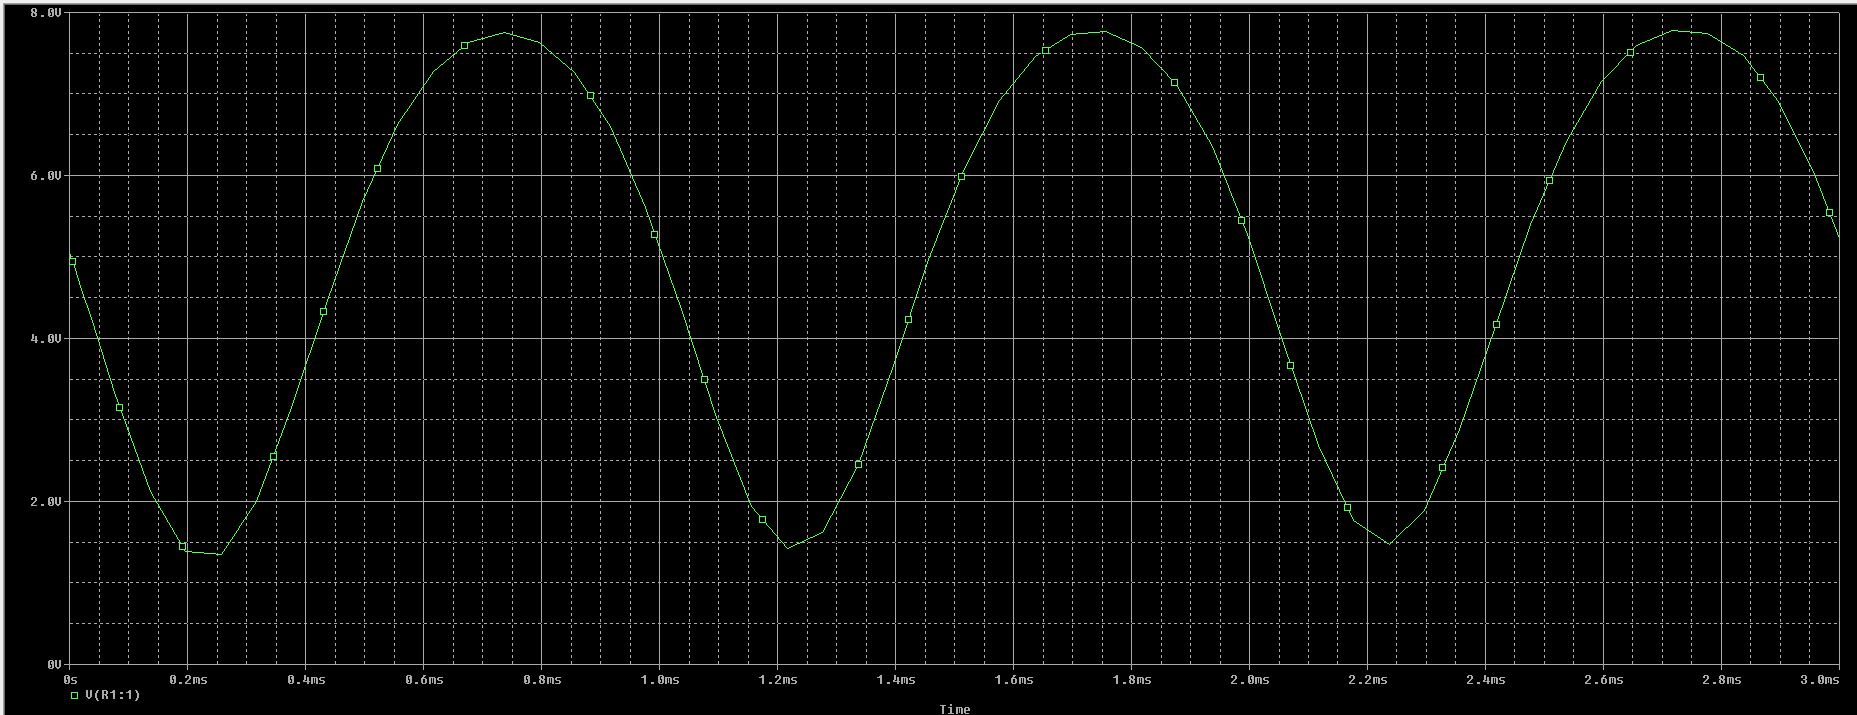
\includegraphics[width=.8\textwidth]{Figures/L4F11}
  \caption{Part 1, $10[\si{\volt}]$ Supply Voltage}
  \label{fig:13}
\end{figure}

\begin{figure}[H]
  \centering
  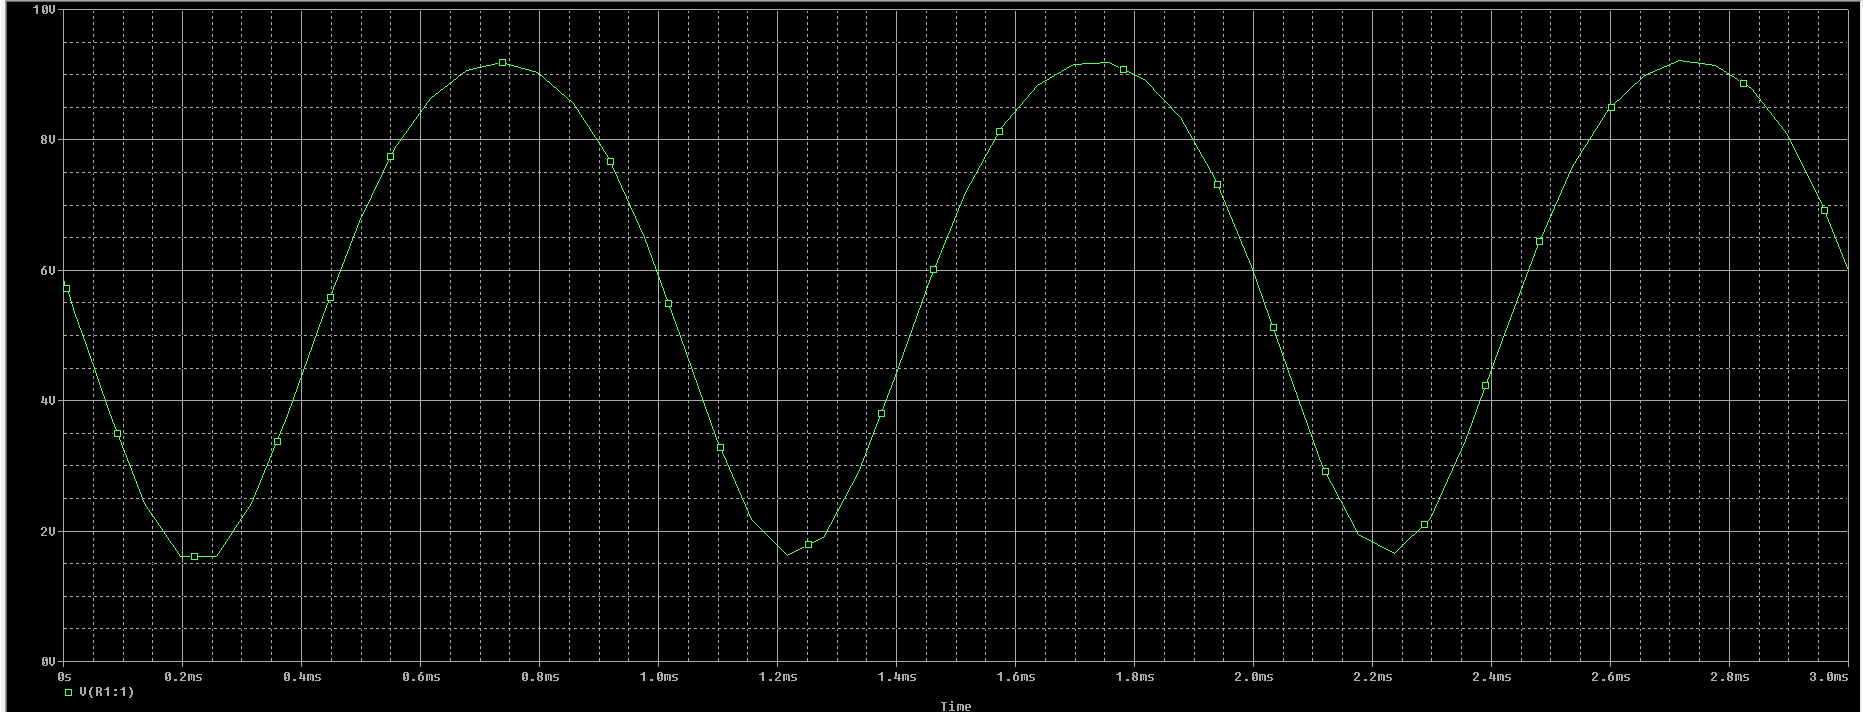
\includegraphics[width=.8\textwidth]{Figures/L4F12}
  \caption{Part 1, $12[\si{\volt}]$ Supply Voltage}
  \label{fig:14}
\end{figure}

We may observe that the supply voltage has a strong affect on the gain; that is, a higher supply voltage generates a greater gain. This is similar to the measurement observed in the physical circuit. Now, let us add a stabilizing resistor to create a circuit whose gain is (more so) independent of the supply voltage. This gives us the following schematic:

\begin{figure}[H]
  \centering
  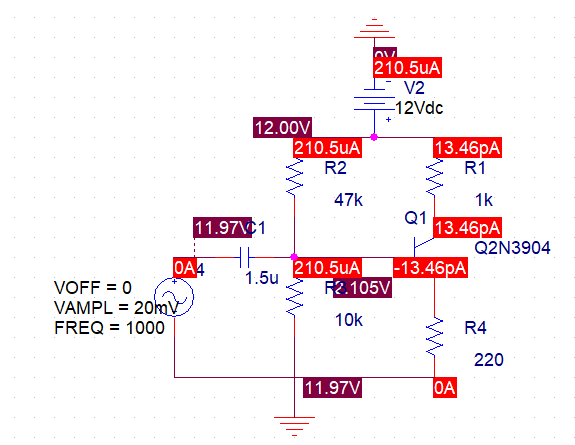
\includegraphics[width=.8\textwidth]{Figures/L4F13}
  \caption{Part 1, Stable Schematic}
  \label{fig:15}
\end{figure}

The stabilization can be seen by re-running the 8,10, and $12[\si{\volt}]$ supply voltage runs to get:

\begin{figure}[H]
  \centering
  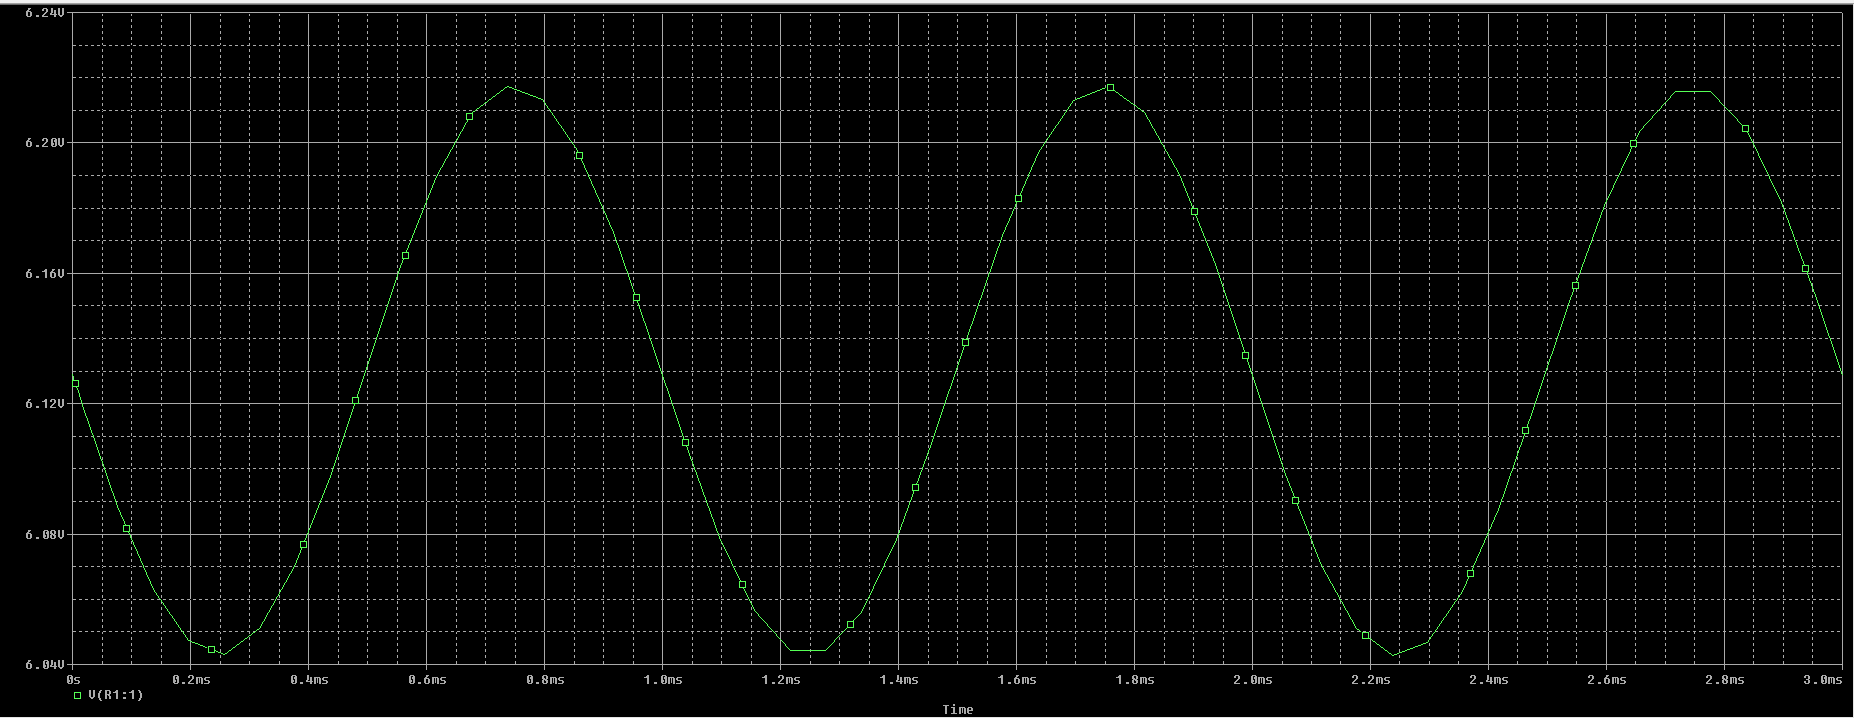
\includegraphics[width=.8\textwidth]{Figures/L4F14}
  \caption{Part 1, $8[\si{\volt}]$ Supply Voltage (Stable)}
  \label{fig:16}
\end{figure}

\begin{figure}[H]
  \centering
  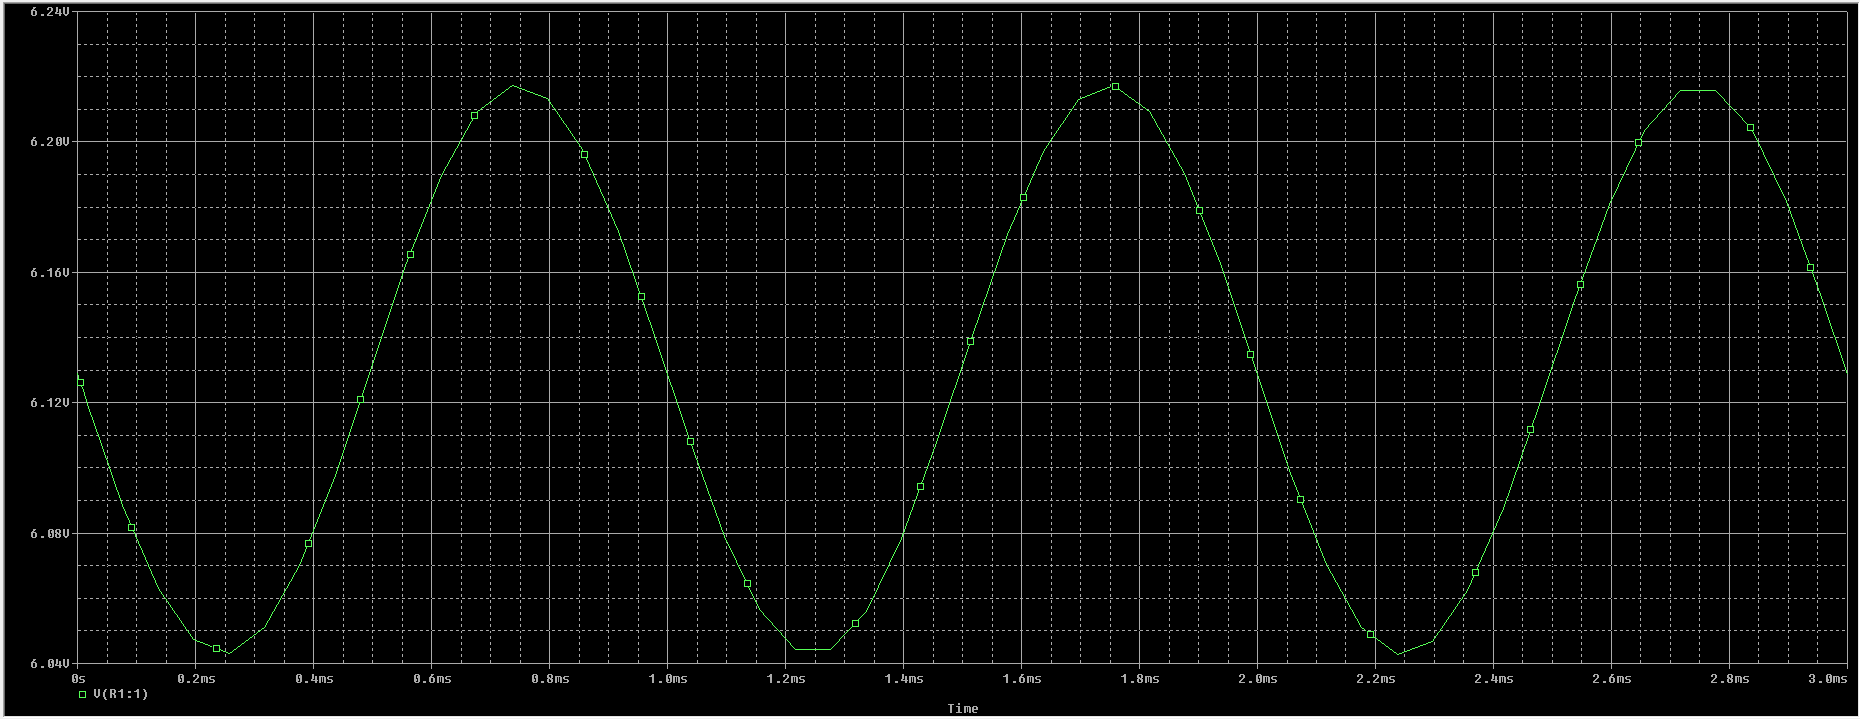
\includegraphics[width=.8\textwidth]{Figures/L4F15}
  \caption{Part 1, $10[\si{\volt}]$ Supply Voltage (Stable)}
  \label{fig:17}
\end{figure}

\begin{figure}[H]
  \centering
  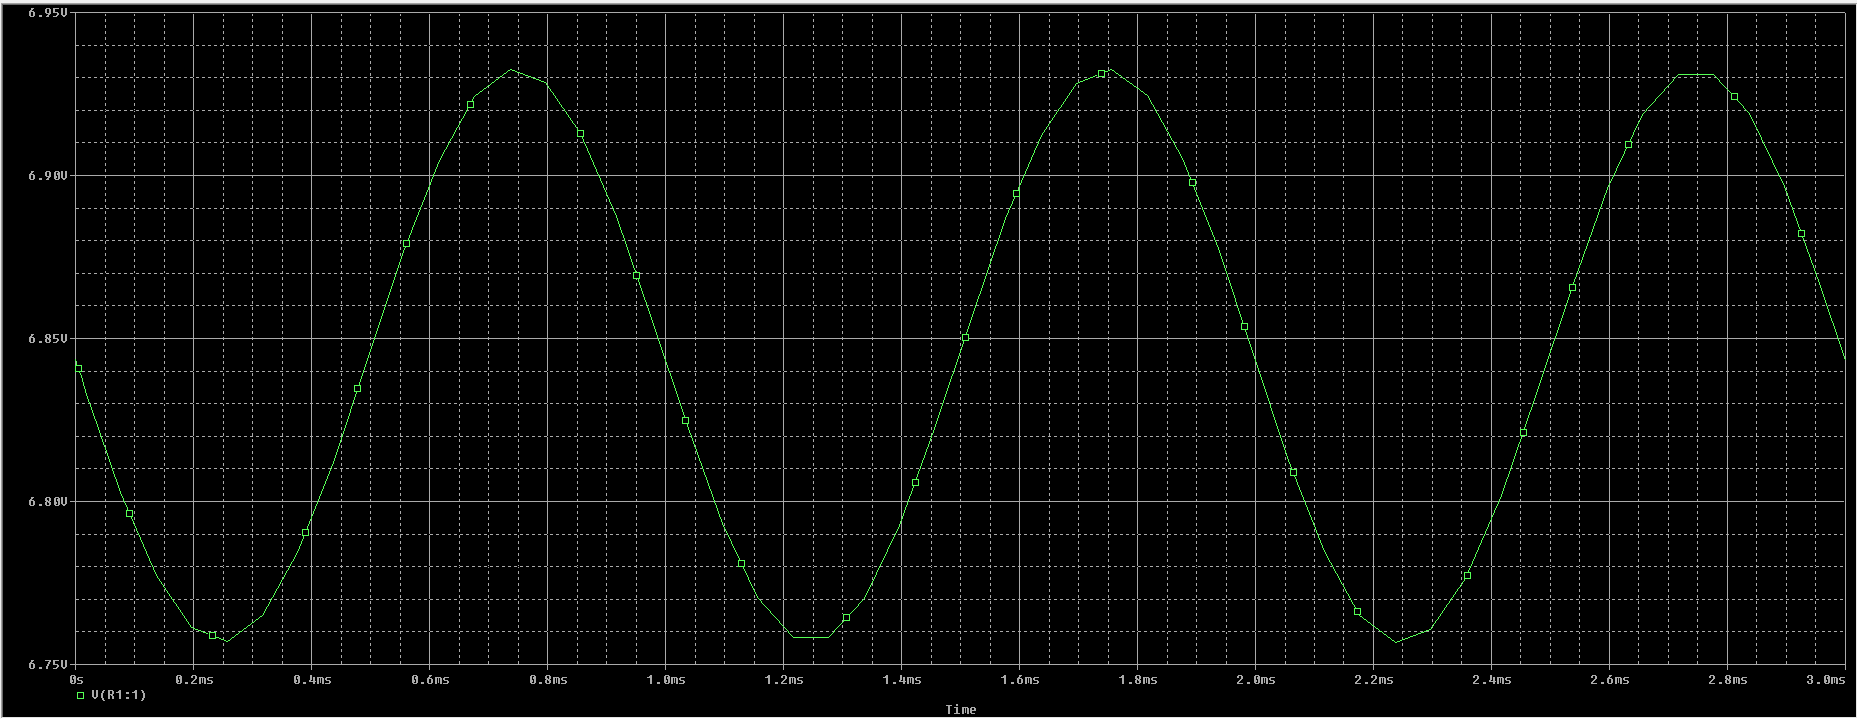
\includegraphics[width=.8\textwidth]{Figures/L4F16}
  \caption{Part 1, $12[\si{\volt}]$ Supply Voltage (Stable)}
  \label{fig:18}
\end{figure}

We can see that, though there is still a correlation, the influence of the supply voltage is drastically reduced. Finally, we may add a gain-boosting capacitor to get:

\begin{figure}[H]
  \centering
  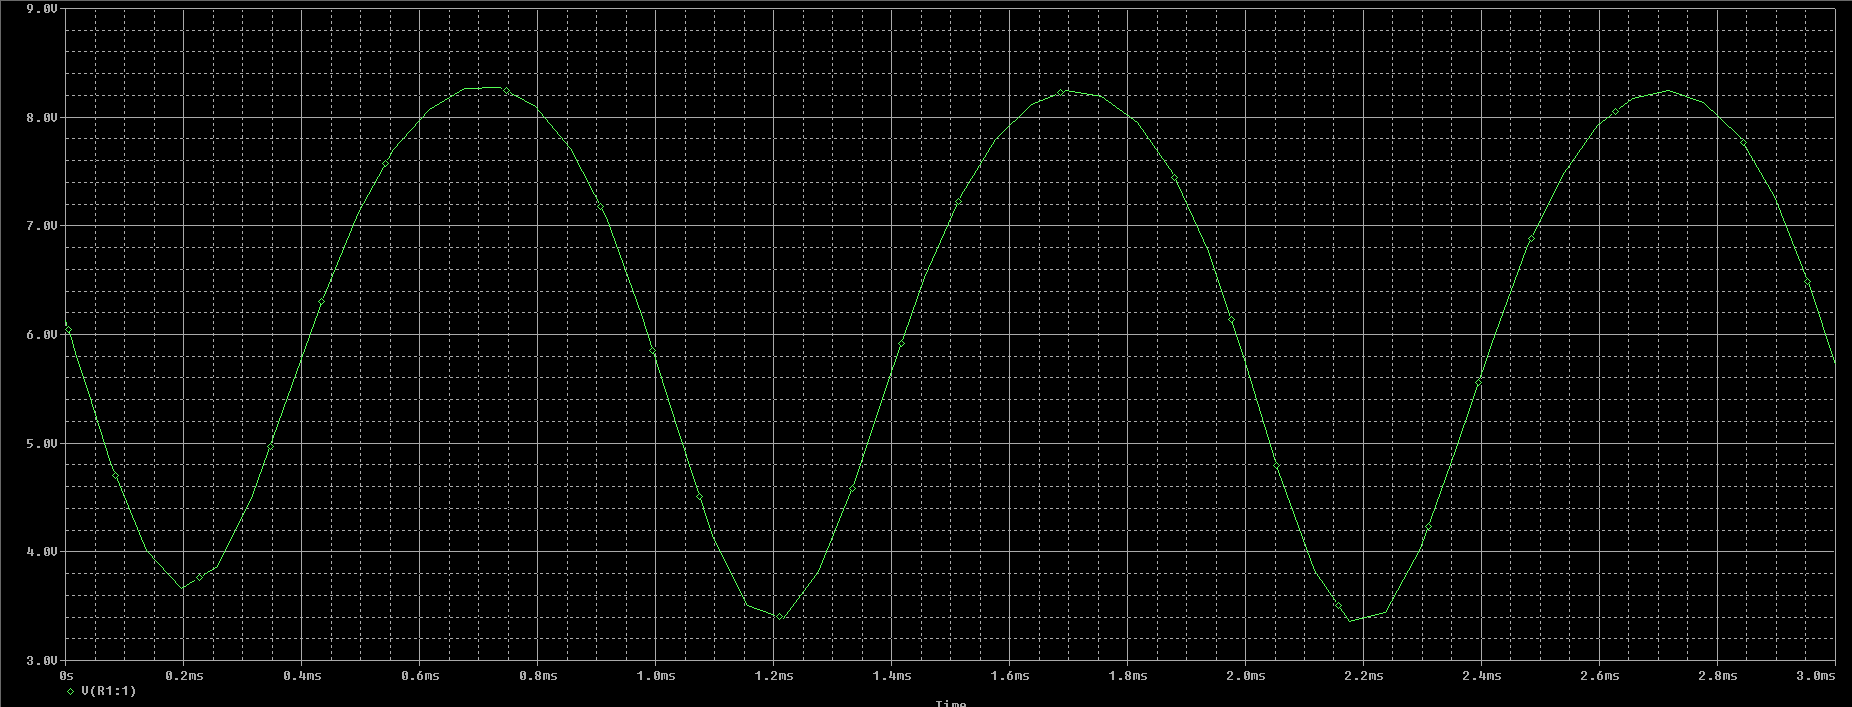
\includegraphics[width=.8\textwidth]{Figures/L4F17}
  \caption{Part 1, Gain-Boosting Capacitor}
  \label{fig:19}
\end{figure}

We may notice that the gain is greater here than the previous plots. We finally may proceed to Part 2, and generate our custom design:

\begin{figure}[H]
  \centering
  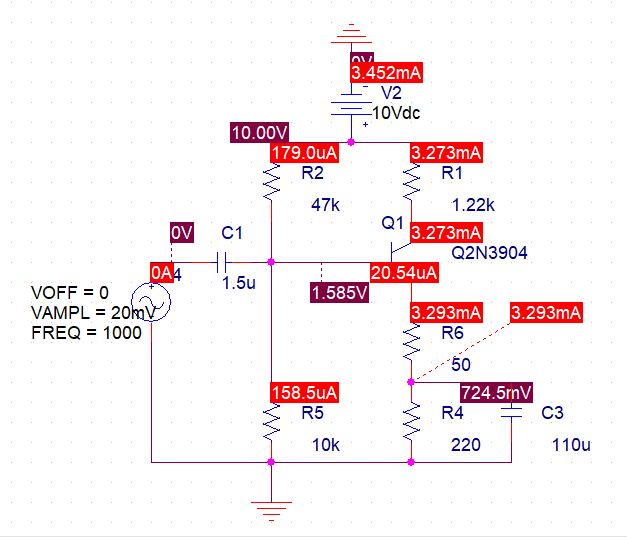
\includegraphics[width=.8\textwidth]{Figures/L4F18}
  \caption{Part 2, Custom Schematic with DC Response}
  \label{fig:20}
\end{figure}

This allows us to see the following output response:

\begin{figure}[H]
  \centering
  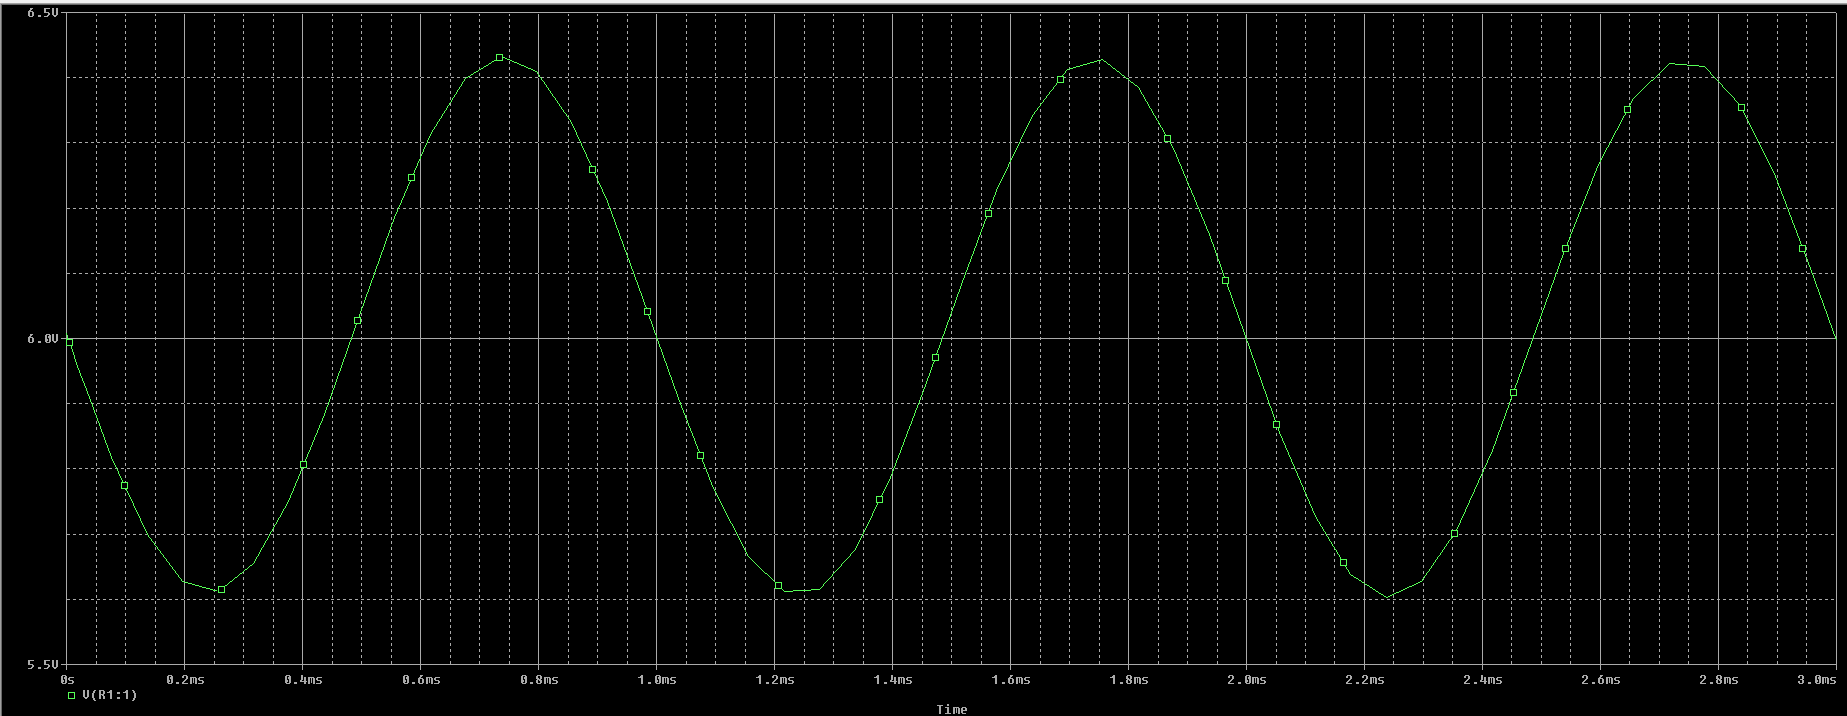
\includegraphics[width=.8\textwidth]{Figures/L4F19}
  \caption{Part 2, Output}
  \label{fig:21}
\end{figure}

\section{Conclusion}

Throughout this laboratory experiment, we observed the function of a common-emitter. This includes, but is not limited to: how to isolate the gain from supply voltage influence, how to isolate the output from DC offset, and understanding why the gain clips at certain voltages.

\end{document}
